%%%% ijcai19.tex

\typeout{IJCAI-19 Instructions for Authors}

% These are the instructions for authors for IJCAI-19.

\documentclass{article}
\pdfpagewidth=8.5in
\pdfpageheight=11in
% The file ijcai19.sty is NOT the same than previous years'
\usepackage{ijcai19}

% Use the postscript times font!
\usepackage{times}
\usepackage{soul}
\usepackage{url}
\usepackage[hidelinks]{hyperref}
\usepackage[utf8]{inputenc}
\usepackage[small]{caption}
\usepackage{graphicx}
\usepackage{amsmath}
\usepackage{booktabs}
\usepackage{algorithm}
\usepackage{algorithmic}
\urlstyle{same}

% the following package is optional:
%\usepackage{latexsym} 

% Following comment is from ijcai97-submit.tex:
% The preparation of these files was supported by Schlumberger Palo Alto
% Research, AT\&T Bell Laboratories, and Morgan Kaufmann Publishers.
% Shirley Jowell, of Morgan Kaufmann Publishers, and Peter F.
% Patel-Schneider, of AT\&T Bell Laboratories collaborated on their
% preparation.

% These instructions can be modified and used in other conferences as long
% as credit to the authors and supporting agencies is retained, this notice
% is not changed, and further modification or reuse is not restricted.
% Neither Shirley Jowell nor Peter F. Patel-Schneider can be listed as
% contacts for providing assistance without their prior permission.

% To use for other conferences, change references to files and the
% conference appropriate and use other authors, contacts, publishers, and
% organizations.
% Also change the deadline and address for returning papers and the length and
% page charge instructions.
% Put where the files are available in the appropriate places.

% If you use natbib package, activate the following three lines:
%\usepackage[round]{natbib}
%\usepackage[numbers]{natbib}
\usepackage{natbib}
%\renewcommand{\bibname}{References}
%\renewcommand{\bibsection}{\subsubsection*{\bibname}}

% If you use BibTeX in apalike style, activate the following line:
%\bibliographystyle{apalike}

%%%%% NEW MATH DEFINITIONS %%%%%

\usepackage{amsmath,amsfonts,bm}
\usepackage{amssymb}
\usepackage{amsthm}
\usepackage{enumitem}
\usepackage{graphicx}
\usepackage{wrapfig}
\usepackage{algorithm}
\usepackage{algorithmic}
\usepackage{picins}
\usepackage{url}
\usepackage[hidelinks]{hyperref}
\usepackage{microtype}
\usepackage[capitalize]{cleveref}
\crefname{prop}{Proposition}{Propositions}
\crefname{thm}{Theorem}{Theorems}
\crefname{lem}{Lemma}{Lemmas}

\newtheorem{thm}{Theorem}
\newtheorem{lem}{Lemma}
\newtheorem{defi}{Definition}
\newtheorem{prop}{Proposition}
\newtheorem{remk}{Remark}

\newcommand{\emp}{\tilde{p}}
\newcommand{\KL}{D_{\mathrm{KL}}}
\newcommand{\softmax}{\mathrm{softmax}}

\DeclareMathOperator*{\argmax}{arg\,max}
\DeclareMathOperator*{\argmin}{arg\,min}
\DeclareMathOperator*{\textmax}{\text{maximize}}

\DeclareMathOperator*\ep{\mathbb{E}}
\DeclareMathOperator\oep{\mathbb{E}}

\newcommand*{\refPi}{\bar{\pi}}
\newcommand*{\optPiRef}{\bar{\pi}_{\tau}^*}
\newcommand*{\cP}{\mathcal{P}}
\newcommand*{\cH}{\mathcal{H}}
\newcommand{\ENT}{\text{ENT}}
\newcommand{\SR}{\text{SR}}
\newcommand{\pithetat}{\pi_{\theta_t}}

\newcommand\scalemath[2]{\scalebox{#1}{\mbox{\ensuremath{\displaystyle #2}}}}

\newcommand*{\subjectto}{\text{subject to}}

\DeclareMathOperator{\sign}{sign}
\DeclareMathOperator{\Tr}{Tr}
\let\ab\allowbreak

\newcommand{\parV}{V_{\phi}}
\newcommand{\parTargetV}{V_{\bar{\phi}}}
\newcommand{\parQ}{Q_{\psi}}
\newcommand{\parPi}{\pi_{\theta}}
\newcommand{\parQone}{Q_{\psi_1}}
\newcommand{\parQtwo}{Q_{\psi_2}}

\def\gD{{\mathcal{D}}}
\def\gO{{\mathcal{O}}}

\def\sE{{\mathbb{E}}}
\def\sR{{\mathbb{R}}}

\def\rvpi{{\boldsymbol{\pi}}}
\def\rvr{{\mathbf{r}}}
\def\rvone{{\mathbf{1}}}

\title{On Principled Entropy Exploration in Policy Optimization}

% Single author syntax
\author{
    Sarit Kraus
    \affiliations
    Department of Computer Science, Bar-Ilan University, Israel \emails
    pcchair@ijcai19.org
}

% Multiple author syntax (remove the single-author syntax above and the \iffalse ... \fi here)
% Check the ijcai19-multiauthor.tex file for detailed instructions

\author{
Jincheng Mei$^{1}$\thanks{Equal contribution}\and
Chenjun Xiao$^{1 *}$\and
Ruitong Huang$^{2}$\and
Dale Schuurmans$^1$\And
Martin M{\" u}ller$^1$
\affiliations
$^1$University of Alberta\\
$^2$Borealis AI Lab\\
\emails
\{jmei2, chenjun\}@ualberta.ca,
ruitong.huang@borealisai.com,
\{daes, mmueller\}@ualberta.ca
}


\begin{document}

\maketitle

\begin{abstract}

Policy optimization is a fundamental problem in reinforcement learning.
In this paper, 
we investigate Reversed Entropy Policy Mirror Descent (REPMD), 
an on-line policy optimization method that improves exploration
while ensuring monotonic progress in a principled objective.
REPMD conducts a form of maximum entropy exploration
within a mirror descent framework,
but alters the policy update with a reversed KL projection.
This modification bypasses undesirable mode seeking behaviour
and avoids premature convergence to sub-optimal policies,
while still achieving strong theoretical properties
such as a policy improvement guarantee.
An experimental evaluation also
shows that this approach significantly improves practical exploration behavior,
surpassing the performance of state-of-the art policy optimization methods
in a range of benchmark tasks.


\end{abstract}

Model-free deep reinforcement learning (RL) has recently been demonstrated its successes in solving a wide range of difficult sequential decision making problems \citep{schulman2015trust,mnih2015human,silver2016mastering}.
Among various deep RL methods one of the core ideas is the policy optimization, which presents the policy search problem as an optimization problem \citep{williams1991function,williams1992simple,sutton1998reinforcement}.
 %, where it aims to find a policy $\pi$ that maximizes the expected reward. 
Policy optimization updates the model by the so-called policy gradient methods, where the policy is modelled by neural networks. 

While the great expressive power of neural networks in deep RL helps in modelling complicated policies, it also introduces the instability and the data inefficiency to the learning algorithms. 
Usually training a deep RL model would require an extensive hyperparameter tuning and a huge, if not impractical, number of sampled trajectories. 
Different from a traditional optimization problem, policy optimization needs to collect its training data from the environment based on its policy, the argument also to be optimized on.
Such interaction may make the performance of the algorithm very sensitive to the policy, thus results in the need of an extensive hyperparameter tuning.
It may also create many local optima, where a lack-of-exploration policy would fail to collect high-reward training data which in turns prevents any further improvement of the policy from useful signals.
Therefore,  a good learning algorithm should have the ability to improve the policy stably, and explore the policy space properly and efficiently to avoid getting trapped in a poor local optimum and discover a good policy quickly.


 %
Many improvements to policy optimization have been proposed in the literature, in both the stability and the data efficiency of the algorithm \citep{peters2010relative,van2015learning,fox2015taming,schulman2015trust,montgomery2016guided,nachum2017bridging,nachum2017trust,tangkaratt2017guide,abdolmaleki2018maximum,haarnoja2018soft}. 
However, a clear gap between their great success in practice and their theoretical analyses remains.
%Despite of its success in practice,  theoretical analyses of these methods have been far limited.
In particular, existing theoretical results typically assume a fairly simple setting, which either ignores the parametrization of the model or only considers linear models. However, it is hard to justify that such assumptions would still hold when using complex approximators with finite representation capacity (restricted by the parameter space constraint), e.g. neural network models.
Such discrepancy between theory and practice has become a hurdle to the wider application of model-free policy gradient methods. 

In this paper, we focus on a more realistic setting where the policy is parametrized as a \emph{non-convex} function in its parameter space. 
We start with the entropy-regularized expected reward as our objective \citep{williams1991function,fox2015taming,schulman2017equivalence,nachum2017bridging,haarnoja2017reinforcement}. 
%While such objective has already been studied in the literature \citep{williams1991function,fox2015taming,schulman2017equivalence,nachum2017bridging,haarnoja2017reinforcement}, our analyses focus on the \emph{non-convex} setting.
We first reformulate this objective as a lift-and-project procedure following the idea of Mirror Descent.
On the one hand, such reformulation makes it easier to analyze the algorithm in the parameter space.
Based on such reformulation, a monotonic improvement guarantee in performance can be proved with a fairly simple proof, even in the non-convex setting.
We also studies its fixed points properties.
On the other hand, such formulation suggests to perform multiple steps of gradient descent on the project step, which leads to our first algorithm, Policy Mirror Descent (PMD). 
 PMD first lifts the policy in the entire policy-simplex, ignoring the constraint induced by its parametrization, then solving a project step by multiple steps of gradient descent to update the policy in the parameter space. 

We then propose additional modifications to mitigate the potential deficiencies of PMD.
Our main algorithm, Reversed Entropy PMD (REPMD),  takes both the entropy and the relative entropy regularizers, and uses a mean seeking direction of KL divergence for projection.
Similar guarantees can also be proved for REPMD but only on a surrogate reward $\SR(\pi)$ rather than the expected reward. 
We further study the properties of $\SR(\pi)$ and provide theoretical and empirical evidences that $\SR$ could serve as a good guidance for learning the policy.
Lastly, we also show how our algorithm can be extended to cooperate with value function approximation, and present its  actor-critic version. 


%Typically the theory assumes a fairly simple setting where either learning happens in the policy space, i.e. the space of all the probability distributions, or the approximator is linear so that the optimization problem is convex. 
\if0
Our first algorithm, Policy Mirror Descent (PMD), is derived from the basic idea of maximizing the relative entropy-regularized expected reward. Such objective has also been used in various reinforcement learning algorithms including \citet{williams1991function,fox2015taming,schulman2017equivalence,nachum2017bridging,haarnoja2017reinforcement}, among others.
As mentioned in \cref{sec:intro}, we focus on analyzing its learning properties in the \emph{non-convex} setting in parameter space.
Our first step in \cref{subsec:revisitTRPO} is to reformulate the 
objective as a lift-and-project procedure following the idea of Mirror Descent. 
We discuss the properties and potential deficiencies of PMD based on such reformulation.
Additional modifications are then proposed  to mitigate these deficiencies in \cref{subsec:repmd}, leading to a new algorithm called Reversed Entropy Policy Mirror Descent (REPMD).
As we will see in \cref{subsec:repmd,subsec:sr}, REPMD enjoys some performance guarantees even in the non-convex setting, e.g. when $\pi_\theta$ is an one-layer-softmax neural network. 
Lastly, although our algorithm is presented purely policy-based, it can be easily extended to cooperate with value function approximation. 
We briefly discussed the actor-critic version of our method in \cref{subsec:repmd_value}.




%In practice, policy based Deep RL is different than a traditional optimization problem, in the sense that the argument to be optimized, i.e. the policy, is also used to collect training data from the environment. 
%Such interaction may lead to lack of exploration, since the learner's policy may get stuck in a local optimum and fail to collect high reward trajectories, preventing any learning from useful signals.  An on-line learning algorithm should have the ability to explore the policy space properly and efficiently, to avoid getting trapped in a locally optima, while discovering the globally optimal policy quickly.
 %Policy optimization has been widely used across reinforcement learning (RL) settings. 

In this paper, we propose a method with a better exploration strategy, such that (a) it retains the exploration efficiency of existing methods; (b) it monotonically increases its chance of exploring trajectories generated by the optimal policies, or evolving closer to the optimal policies. Our proposed method Reversed Entropy Policy Mirror Descent (REPMD), takes both the entropy and relative entropy regularizers. Unlike common policy gradient based methods, REPMD is in a two-stage manner.  REPMD first updates the policy in the entire policy-simplex, ignoring the constraint induced by its parametrization, then a projection step is performed to update the policy in the parametrized policy space. Such a two-stage update guarantees REPMD to increase performance monotonically. The proposed REPMD method is then justified from both theoretical and empirical perspectives.


The rest of the paper is organized as follows. After introducing exploration of RL in \cref{sec:exploration_in_policy_optimization}, we propose the REPMD method in \cref{sec:reversed_emtropy_policy_mirror_descent}. We provide the analysis for the monotonically increasing performance property of REPMD in \cref{sec:reversed_emtropy_policy_mirror_descent}, and conduct experiments to validate our algorithm in \cref{sec:experiments}. Some related work is discussed in \cref{sec:related_work}, and the conclusion and directions for future work are presented in \cref{sec:conclusion_and_future_work}.
\fi
\subsection{Notations and Problem Setting}
\label{subsec:notations_and_settings}
For simplicity, we only consider finite horizon reinforcement learning settings with finite state and action spaces. 
The behavior of an agent is modelled by a policy $\pi(a|s)$, which estimates a probability distribution over a finite set of actions given an observed state. 
At each time step $t$, the agent takes an action $a_t$ by sampling from $\pi(a_t | s_t)$. The environment then returns a reward $r_t = r(s_t, a_t)$ and the next state $s_{t+1} = f(s_t, a_t)$, where $f$ is the transition function not revealed to the agent.
Given a trajectory, a sequence of states and actions $\rho=(s_1, a_1, \dots, a_{T-1}, s_T)$, the policy probability and the total reward of $\rho$ are defined as $\pi(\rho) = \prod_{t=1}^{T-1} \pi(a_t| s_t)$ and $r(\rho) = \sum_{t=1}^{T-1} r(s_t, a_t)$. 
Given a set of parametrized policy functions $\pi_\theta \in \Pi$, policy optimization aims to search the optimal policy $\pi_\theta^*$ by maximizing the expected reward,
\begin{equation}
\label{max_expected_reward}
\begin{split}
\pi_\theta^* \in \argmax_{\pi_\theta \in \Pi}{ \ep\limits_{\rho \sim \pi_\theta}{r(\rho)} },
\end{split}
\end{equation}

We use $\Delta \triangleq \{ \pi | \sum_{\rho}{\pi(\rho)} = 1, \pi(\rho) \ge 0, \forall \rho \}$ to refer to the probabilistic simplex over all possible trajectories. 
Without loss of generality, we also assume that the state transition function is deterministic, and the discount factor $\gamma = 1$.
The same simplification is also assumed in \citet{nachum2017improving}. 
Results for stochastic state transition function are presented in ******.

 %parameterizatio

\section{Policy Mirror Descent}
\label{subsec:revisitTRPO}

\newcommand{\real}{\mathbb{R}}


We begin with the development of the Policy Mirror Descent (PMD) strategy,
which will form the basis for our subsequent algorithms and their analyses.
As mentioned in the introduction, our analysis of this and subsequent methods
focuses on the \emph{non-convex} setting.

Consider the following local optimization problem:
given a \emph{reference policy} $\refPi$ (usually the current policy), 
maximize the proximal regularized expected reward,
using relative entropy as the regularizer:
\begin{equation}
\label{eq:max_expected_reward_plus_relative_entropy}
\pi_{\theta} = \argmax\limits_{\pi_\theta \in \Pi} { \ep\limits_{\rho \sim \pi_\theta}{  r(\rho)  - \tau \KL(\pi_\theta \| \refPi) } }.
\end{equation}
Relative entropy regularization has been widely investigated in
online learning and optimization
\citep{nemirovskii1983problem,beck2003mirror},
primarily as a component of the mirror descent algorithm.
Observe that when $\refPi$ is the uniform distribution,
\cref{eq:max_expected_reward_plus_relative_entropy}
reduces to entropy regularized expected reward.
It is important to note that,
since we are interested in the non-convex setting
and only assume that
$\pi$ is parametrized as a smooth
function of $\theta \in \real^d$,
$\Pi$ is generally a non-convex subset of the simplex.
Therefore, 
\cref{eq:max_expected_reward_plus_relative_entropy}
is a difficult constrained optimization problem.

A useful way to decompose this optimization
is to consider an alternating lift-and-project procedure
that isolates the different computational challenges.
%
{\small
\begin{equation}
\label{eq:pmd}
\begin{aligned}
&\text{\bf (Project)} \quad \argmin\limits_{\pi_\theta \in \Pi}{\KL( \pi_\theta \| \bar{\pi}_{\tau}^* )}, \\
&\text{\bf (Lift)}  \quad  \text{where}\ \ \bar{\pi}_{\tau}^* =  \argmax\limits_{\pi \in \Delta}{ \ep\limits_{\rho \sim \pi}{  r(\rho)  - \tau \KL(\pi \| \refPi) } }.
\end{aligned}
\end{equation}
}
Crucially, the reformulation \cref{eq:pmd} remains equivalent to the
original problem \cref{eq:max_expected_reward_plus_relative_entropy},
in that it preserves the same set of solutions,
as established in \cref{prop:mirrordescent_projection}.

\begin{prop}
\label{prop:mirrordescent_projection}
Given a \emph{reference policy} $\refPi$,
{\small
\begin{equation*}
	\argmax\limits_{\pi_\theta \in \Pi} { \ep\limits_{\rho \sim \pi_\theta}{  r(\rho)  - \tau \KL(\pi_\theta \| \refPi) } } 
 = \argmin\limits_{\pi_\theta \in \Pi}{ \KL(\pi_\theta \| \bar{\pi}_\tau^*) }.
\end{equation*}
}
\end{prop}
Note that this result holds even for the non-convex setting.
%
The reformulation \cref{eq:pmd} immediately leads to our PMD algorithm:
Lift the current policy $\pi_{\theta_t}$ to $\bar{\pi}_\tau^*$,
then perform multiple steps of gradient descent in the Project Step
to update $\pi_{\theta_{t+1}}$.%
%
\footnote{
%To estimate this gradient one would need to use self-normalized importance sampling \cite{owen2013monte}.
We omit the details here since PMD is not our main algorithm;
similar techniques can be found in the implementation of REPMD. 
% in cref-tbd.
}
%Note that vanilla gradient descent methods for TRPO can be interpreted as performing only one step gradient descent for the project step. \todor[]{Is it correct?} 

When $\Pi$ is a convex set, one can show that PMD asymptotically converges to the optimal policy \citep{nemirovskii1983problem,beck2003mirror}. 
The next proposition shows that despite the non-convexity of $\Pi$,
PMD still enjoys desirable properties.

\begin{prop}
\label{prop:monoto_policymirrordescent}
Let $\pi_{\theta_{t}}$ denote the policy at step $t$ of
the update sequence.
Then PMD satisfies the following properties for an arbitrary 
parametrization of $\pi$.
\begin{enumerate}
	\item {\bf (Monotonic Improvement)} 
	%The sequence of policies learned by TRPO is guaranteed to be monotonically improved:
	If the Project Step $\min\limits_{\pi_\theta \in \Pi}{\KL( \pi_\theta \| \bar{\pi}_{\tau}^* )}$ can be globally solved, then
	 \begin{equation*}
	\oep_{\rho \sim \pi_{\theta_{t+1}}}{r(\rho)} - \oep_{\rho \sim \pi_{\theta_{t}}}{  r(\rho)} \ge 0.
	\end{equation*}
	\item {\bf (Fixed Points)} If the Project Step is optimized by gradient descent, then the fixed points of PMD are the 
	 stationary points of $\oep_{\rho \sim \pi_\theta}{  r(\rho)}$. 
\end{enumerate}
\end{prop}
Despite these desirable properties, 
\cref{prop:monoto_policymirrordescent}
relies on the condition that the Project Step in PMD is solved to
global optimality.
It is usually not practical to achieve such a stringent requirement
when $\pi_\theta$ is not convex in $\theta$,
limiting the applicability of \cref{prop:monoto_policymirrordescent}.

Another shortcoming with this naive strategy is 
that PMD typically gets trapped in poor local optima.
Indeed, while the relative entropy regularizer help prevent
a large policy update, it also tends to limit exploration.
Moreover, minimizing the KL divergence
$\KL(\pi_\theta \| \bar{\pi}_\tau^*)$
is known to be \emph{mode seeking} \citep{kevin2012machine},
which can lead to mode collapse during the learning process.
%Indeed, if the current policy has $0$ probability on some actions, the relative entropy term and the mode seeking projection will prevent the algorithm to explore these actions anymore.
Once a policy $\bar{\pi}_\tau^*$ has lost important modes,
learning can easily become trapped at a sub-optimal policy.
Unfortunately, at such points,
the relative entropy regularizer does not encourage further exploration.








%\subsection{Reversed Entropy Policy Mirror Descent}
\section{Reversed Entropy Policy Mirror Descent}
\label{subsec:repmd}

We present our main algorithm Reversed Entropy Policy Mirror Descent (REPMD) in this section. 


We now present REPMD that introduces two modifications to PMD to overcome its aforementioned potential deficiencies.
The first modification is an additional entropy regularizer to the lift step to encourage the exploration of the algorithm, 
and the second one is using a reversed \emph{mean seeking} direction of KL divergence for the project step.
In particular, REPMD solves the following optimization problem to update the policy $\pi_{\theta_{t+1}}$:
\begin{equation}
\label{eq:repmd}
\begin{split}
\text{\bf (Project Step)} \quad  &\argmin\limits_{\pi_\theta \in \Pi}{\KL(\bm{ \bar{\pi}_{\tau,\tau^{\prime}}^* \| \pi_\theta }) }, \\
\text{\bf (Lift Step)} \quad  & \text{where}\ \ \bar{\pi}_{\tau,\tau^{\prime}}^*  =  \argmax\limits_{\pi \in \Delta}{ \ep\limits_{\rho \sim \pi}{  r(\rho)  - \tau \KL(\pi \| \pi_{\theta_t}) + \bm{\tau^{\prime} \cH(\pi)} }}.
\end{split}
\end{equation}
%, leading to our new algorithm.
The idea of optimizing the reverse direction of KL divergence has proven to be effective for structured prediction and reinforcement learning in previous work, such as reward augmented maximum likelihood \citep{norouzi2016reward} and UREX \citep{nachum2017improving}.
Its \emph{mean seeking} behavior would further encourage the exploration of the algorithm.
As we will see in \cref{sec:experiments}, REPMD outperforms PMD significantly in our experiments. 

\cref{thm:monotonically_increasing_sr_property} shows that REPMD also enjoys similar desirable properties in the non-convex setting, but on a surrogate reward $\SR(\pi_\theta)$.
\begin{thm}
\label{thm:monotonically_increasing_sr_property}
Assume that $\pi_{\theta_{t}}$ is the update sequence. REPMD satisfies the following properties for an arbitrary parametrization of $\pi$.
\begin{enumerate}
	\item {\bf (Monotonic Improvement Guarantee)} 
	%The sequence of policies learned by TRPO is guaranteed to be monotonically improved:
	If the project step $\KL( \bar{\pi}_{\tau,\tau^{\prime}}^* \| \pi_\theta )$ can be solved globally optimally,, then 
	\begin{equation*}
	\SR(\pi_{\theta_{t+1}}) - \SR(\pithetat)\ge 0,
	\end{equation*}
	where
	\begin{equation}
	\label{eq:SR}
	\SR(\pi_\theta) \triangleq (\tau + \tau^{\prime})\log{ \sum_{\rho}{ \exp\left\{ \frac{r(\rho) + \tau \log{\pi_\theta(\rho)} }{\tau + \tau^{\prime}} \right\} }}.
	\end{equation}
	\item  {\bf (Global Optimum Guarantee)} If the project step can be solved globally optimally, then $ \pi_{\theta_{t}}$ converges to the global optimum $\pi^*$, i.e. 
	\[
	\SR(\pi^*) \ge  \SR(\pi), \quad \forall \pi\in\Pi.
	\]
	\item {\bf (Fixed points)} Assume that the project step is optimized by gradient descent, then the fixed points of REPMD are the 
	stationary points of the expected reward $\SR(\pi_\theta)$. 
\end{enumerate}
%Theorem \ref{thm:monotonically_increasing_sr_property} guarantees the monotonic improvement on $\text{SR}(\pi)$, thus implies that 
%the fixed points of REPMD have a correspondence with the stationary point of $\text{SR}(\pi_\theta)$. \todor[]{Why?}
\end{thm}

Can the project step be solved optimally? It is straightforward that when $\pi(\theta) = \theta \in \Delta$, the project step is a convex optimization problem, and thus can solved optimally.
Furthermore, as shown in \cref{prop:solvableprojection}, 
for the one-layer-softmax neural network $\pi$, the project step $\KL( \bar{\pi}_{\tau,\tau^{\prime}}^* \| \pi_\theta )$ can also be solved globally optimally.
%reversing the direction of the KL divergence makes the projection step solvable even for the one-layer-softmax neural network $\pi$, thus guarantees the desirable properties in practice.
\begin{prop}
	\label{prop:solvableprojection}
	Assume $\pi_\theta(s) = \softmax(\phi_s^{\top}\theta)$. Given a reference policy $\refPi$, the projection step $\min\limits_{\theta \in \mathbb{R}^d}{\KL(\refPi \| \pi_\theta)}$ is convex in $\theta$.
\end{prop}


%\subsubsection{Behavior of $\SR(\pi)$}
\subsection{Behavior of $\SR(\pi)$}
\label{subsec:sr}
\cref{thm:monotonically_increasing_sr_property} only shows the desirable properties on $\SR(\pi)$.
In this section we present some theoretical and empirical evidences that $\SR(\pi_\theta)$ is a reasonable surrogate that may actually provide good guidance to the learning. 
In fact, by properly adjusting the two temperature parameters $\tau$ and $\tau^{\prime}$, $\SR(\pi_\theta)$ recovers several existing performance measures, as shown in \cref{prop:sr}.
\begin{prop}
\label{prop:sr}
$\SR(\pi_\theta)$ satisfies the following properties:
\begin{enumerate}[label=(\roman*)]
	\item  $\SR(\pi_\theta) \to \max_{\rho}{r(\rho)}$, as $\tau \to 0, \tau^{\prime} \to 0$.
	\item $\SR(\pi_\theta) \to \ep_{\rho \sim \pi_\theta}{r(\rho)}$, as $\tau \to \infty, \tau^{\prime} \to 0$. 
\end{enumerate}	
\end{prop}
\begin{remk}
	Note that $\text{SR}(\pi_\theta)$ also resembles ``softmax value function'' that appeared in value based RL \citep{nachum2017bridging,haarnoja2018soft,ding2017cold}. The standard soft value can be recovered by $\text{SR}(\pi_\theta)$ as a special case when $\tau = 0$ or $\tau'=0$. 
	%\todor[]{But \cref{prop:sr} says that $SR(\pi)$ converges to $max_\rho$ when $\tau$ and $\tau^\prime$ are 0?}
\end{remk}

According to \cref{prop:sr}, one should gradually decrease $\tau^{\prime}$ to reduce the level of exploration as sufficient reward landscape information has been collected during the learning process. Now we can make different choices for $\tau$, depending on the policy constraint set $\Pi$.
%\begin{remk}
%\label{small_tau_choices}
Given $\tau^{\prime} \to 0$ and the reward landscape has been sufficiently explored,
the constructed unconstrained policy $\bar{\pi}_{\tau,\tau^{\prime}}^* \to \pi^*$ as $\tau \to 0$, where $\pi^*$ is the global deterministic optimal policy. 
Therefore, in the project step $\pi_\theta$ is obtained by directly projecting $\pi^*$ into $\Pi$. When the policy constraint $\Pi$ has nice properties, such as convexity, that support good behavior of KL projection, $\pi_\theta$ may achieve good performance.
However, in practice, $\Pi$ is typically non-convex. Setting $\tau \to 0$ might not work very well, since directly projecting $\pi^*$ into $\Pi$ does not always lead to a $\pi_\theta$ with large expected reward.
\begin{wrapfigure}{r}{0.56\textwidth}
	\begin{minipage}{0.56\textwidth}
		\begin{algorithm}[H]
			\caption{\label{alg:repmd}  The REPMD algorithm}
			\begin{algorithmic}[1]
				\INPUT $\tau, \tau', K$
				\OUTPUT  Policy $\pi_\theta$
				\STATE Random initialized $\pi_{\theta_1}$;
				\FOR { $t=1,2,\ldots, T$ }
				\STATE Set $\refPi = \pithetat$;
				\REPEAT 
				\STATE Sample a mini-batch of $K$ trajectories from $\refPi$;
				\STATE Compute the gradient according to \cref{eq:gradient_estimator};
				\STATE Update $\pi_{\theta_{t+1}}$ by the gradient;
				\UNTIL converged or reach max\_iter;
				\ENDFOR
				\STATE Return $\pi_{\theta_T}$.
			\end{algorithmic}
		\end{algorithm}
	\end{minipage}
\end{wrapfigure}


On the other hand, as $\tau \to \infty$ the stationary point set of $\SR(\pi_\theta)$ will approach the stationary point set of $\sum_{\rho}{ \pi_\theta(\rho) r(\rho) }$.
%There exists an ideal sequence of $\tau$ values and $\tau \to \infty$ that make $\pi_\theta$ finally converge to $\pi_\theta^* \in \argmax_{\pi_\theta}{ \sum_{\rho}{\pi_\theta(\rho) r(\rho)} }$, i.e., the optimal policy in $\Pi$ with highest expected reward, recovering the target of policy optimization \cref{max_expected_reward}. \todor[]{Why?}
We empirical investigate the behavior of $\SR{\pi}$ on a simulation setting, as shown in \cref{fig:srsimulation}.
\todor[]{Add the simulation setting in the caption of the figure.}
Note that there is a poor local maximum for $\theta <0$, where naive gradient method will converge to if $\theta$ is initialized on the left. 
When $\tau = 0.2$, the reward landscape of $SR(\pi)$ can guide the learning of $\theta$ to converges to the neighbourhood of $0$, thus helps avoid the poor local maximum. Later in the training when $\tau$ increases to $10$, $SR(\pi)$ recovers the true expected reward landscape, where $\theta$ will converge to a good local , if not the global, maximum.
While a simulation result may be still preliminary, it suggests that $\SR(\pi)$ could be a good guidance for maximizing the true expected reward in some cases.
Further investigation on the behavior of $\SR(\pi)$
%and a principled way to find such an ideal sequence of $(\tau,\tau')$ 
is left for future work.
\if0
Using very small $\tau$ value, i.e., $\tau \to 0$, given $\tau^{\prime} \to 0$ and the reward landscape has been sufficiently explored, the constructed unconstrained policy $\bar{\pi}_{\tau,\tau^{\prime}}^* \to \pi^*$, where $\pi^*$ is the global deterministic optimal policy. Solving the projection $\pi_\theta \leftarrow \argmin_{\pi_\theta \in \Pi}{\KL(\bar{\pi}_{\tau,\tau^{\prime}}^* \| \pi_\theta}) \approx \argmin_{\pi_\theta \in \Pi}{\KL(\pi^* \| \pi_\theta})$, we actually obtain $\pi_\theta$ policy by directly projecting $\pi^*$ into $\Pi$. When the policy constraint $\Pi$ has additional nice properties, such as convexity, that support good behavior of KL projection, this should be a good choice.
%\end{remk}
However, in practice, $\Pi$ is typically non-convex, even when $\pi_\theta$ is parameterized by a linear function approximator, let alone more complex function approximations like a neural network. In such cases, the small $\tau$ value suggested in Remark \ref{small_tau_choices} might not work very well, since directly projecting $\pi^*$ into $\Pi$ might not always lead to a $\pi_\theta$ with large expected reward.

\begin{remk}
\label{large_tau_choices}
	Given $\tau^{\prime} \to 0$ and a sufficiently explored reward landscape, as $\tau \to \infty$, the stationary point set of $\SR(\pi_\theta)$ will approach the stationary point set of $\sum_{\rho}{ \pi_\theta(\rho) r(\rho) }$.
\end{remk}
 
Remark \ref{large_tau_choices} indicates that during learning, $\pi_\theta$ may get stuck around some local maximum of $\SR(\pi_\theta)$, and increasing the $\tau$ value will lead to a different contour of $\SR(\pi_\theta)$, which might help $\pi_\theta$ escape to alternative local maxima. There exists an ideal sequence of $\tau$ values and $\tau \to \infty$ that make $\pi_\theta$ finally converge to $\pi_\theta^* \in \argmax_{\pi_\theta}{ \sum_{\rho}{\pi_\theta(\rho) r(\rho)} }$, i.e., the optimal policy in $\Pi$ with highest expected reward, recovering the target of policy optimization \cref{max_expected_reward}. A principled way to find such an ideal sequence of $\tau$ is under investigation.
 \fi
 
\begin{figure*}[t]
\begin{center}
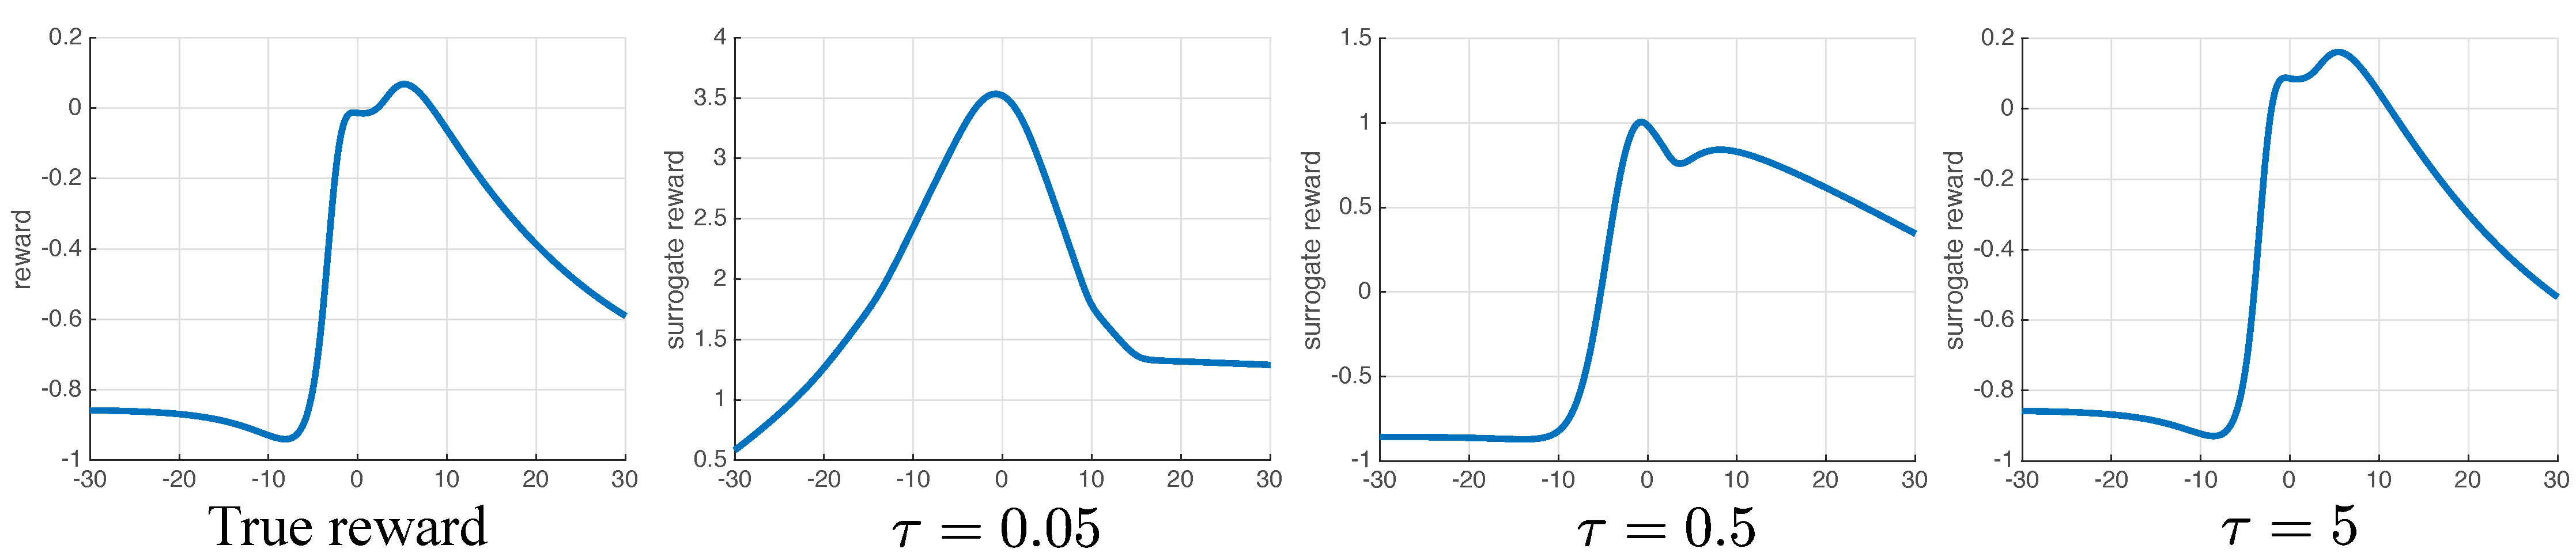
\includegraphics[width=1.0\linewidth]{./sr_simulation.pdf}
\end{center}
\caption{
Simulation result for true reward landscape and $\SR(\pi)$ with different value of $\tau$.} 
\label{fig:srsimulation}
\end{figure*}
 
\subsection{Learning }
\label{subsec:learning}
\todor[]{Maybe move this section to Appendix}
We now discuss the implementation details of REPMD. The full algorithm is presented in \cref{alg:repmd}.
Despite of its non-convexity, it can be verified that the lift step has an analytic solution
\begin{equation}
\label{eq:pitautauprime}
\bar{\pi}_{\tau,\tau^{\prime}}^*(\rho) \triangleq \frac{\refPi(\rho) \exp\left\{ \frac{r(\rho)-\tau^{\prime} \log \refPi(\rho) }{ \tau+\tau^{\prime}} \right\}}{ \sum_{\rho^{\prime}}{\refPi(\rho^{\prime}) \exp\left\{ \frac{r(\rho^{\prime})-\tau^{\prime} \log \refPi(\rho^{\prime})}{ \tau+\tau^{\prime}} \right\} } }.
\end{equation}
%First note that the \emph{unconstrained optimal policy} $\bar{\pi}_{\tau,\tau^{\prime}}^*$ in (\ref{eq:repmd}) has a closed form expression.
%To see that, note that $\argmin\nolimits_{\pi_\theta \in \Pi}\KL(\bar{\pi}_{\tau,\tau^{\prime}}^* \| \pi_\theta) = \argmin\nolimits_{\pi_\theta \in \Pi} \ep_{\rho \sim \bar{\pi}_{\tau,\tau^{\prime}}^* }  - \log \pi_\theta(\rho)$.
The project step in \cref{eq:repmd}, $\min\nolimits_{\pi_\theta \in \Pi}{\KL(\bm{ \bar{\pi}_{\tau,\tau^{\prime}}^* \| \pi_\theta }) }$, can be optimized via stochastic gradient descent, given that one can sample trajectories from $\bar{\pi}_{\tau,\tau^{\prime}}^*$ to estimate its gradient. To see this, note that $\argmin\nolimits_{\pi_\theta \in \Pi}\KL(\bar{\pi}_{\tau,\tau^{\prime}}^* \| \pi_\theta) = \argmin\nolimits_{\pi_\theta \in \Pi} \ep_{\rho \sim \bar{\pi}_{\tau,\tau^{\prime}}^* }  - \log \pi_\theta(\rho)$. The next theorem shows that sampling from $\bar{\pi}_{\tau,\tau^{\prime}}^*$ can be done using self-normalized importance sampling \citep{owen2013monte}, following the idea of UREX \citep{nachum2017improving}.
\begin{thm}
\label{thm:repmdgradientestimate}
Let $\omega_k = \frac{r(\rho_k) - \tau^{\prime} \log{\refPi(\rho_k)} }{\tau + \tau^{\prime}}$. Given $K$ \emph{i.i.d.} samples $\{\rho_1, \dots, \rho_K\}$ from the \emph{reference policy} $\refPi$, we have the following unbiased gradient estimator,
\begin{equation}
\label{eq:gradient_estimator}
	\nabla_{\theta} \KL(\bar{\pi}_{\tau,\tau^{\prime}}^* \| \pi_\theta)\approx -\sum\limits_{k=1}^K{ \frac{ \exp\left\{ \omega_k \right\} }{ \sum_{j=1}^K{ \exp\left\{ \omega_j \right\}}} \nabla_{\theta} \log{\pi_\theta(\rho_k)} },
\end{equation}
%	where 
%	\[
%	\omega_k = \frac{r(\rho_k) - \tau^{\prime} \log{\refPi(\rho_k)} }{\tau + \tau^{\prime}}.
%	\] 
\end{thm}



















%\subsection{Cooperate with Value Function Approximation}
%\section{Combining REPMD with Value Function Approximation}
\section{An Actor-Critic Extension}
\label{subsec:repmd_value}

\newcommand{\parV}{V_{\phi}}
\newcommand{\parTargetV}{V_{\bar{\phi}}}
\newcommand{\parQ}{Q_{\psi}}
\newcommand{\parPi}{\pi_{\theta}}
\newcommand{\parQone}{Q_{\psi_1}}
\newcommand{\parQtwo}{Q_{\psi_2}}


The last part of this section is a nature extension of REPMD with value function approximation, named as Policy Mirror Actor-Critic (PMAC) . 



It has been shown that the data efficiency of policy-based methods can be improved by a critic in general. 
In this section, we present an actor-critic version of REPMD, named as Policy Mirror Actor Critic (PMAC). 
%We consider an infinite trajectory $\rho$ while keeping the discounted factor $\gamma=1$ for simplicity. All the results have no difficulty to extend to a  general value of $\gamma$. 
Given a reference policy $\refPi$ and an initial state $s$, recall that the objective in the Lift Step is 
\[
\gO_{\text{REPMD}}(\pi, s) =   \ep\limits_{\rho \sim \pi}{  r(\rho)  - \tau \KL(\pi \| \refPi) + \tau^{\prime} \cH(\pi)}, 
\]
where $\rho=  (s_1 = s, a_1, s_2, a_2, \ldots)$.
 To cooperate with value function approximation, we will need to derive the temporal consistency for this objective, as follows. 
 \[
 \gO_{\text{REPMD}}(\pi, s) = \E_{a\sim \pi(\cdot \vert s)} \left[ r(s,a) + \gO_{\text{REPMD}}(\pi, s')  + \tau \log \refPi(a|s) - \left(\tau+ \tau' \right) \log \pi(a|s) \right]. 
 \]
%We first alter our definitions of policy and value functions to include the KL and entropy regularization. Given a reference policy $\refPi(a|s)$, we consider the entropy regularized maximum reward objective, \todoc[]{add the trust-pcl reference here or just discuss it in related work?}
%\begin{equation*}
%\gO_{\text{RELENT}}(\pi, s) = \E_{a\sim \pi} \left[ r(s,a) + \gO_{\text{RELENT}}(\pi, s')  + \tau \log \refPi(a|s) - \left(\tau+ \tau' \right) \log \pi(a|s) \right] \\
%\label{relent-obj}
%\end{equation*}
Let $\bar{\pi}_{\tau,\tau^{\prime}}^* (\cdot|s) = \argmax_{\pi} \gO_{\text{REPMD}}(\pi, s) $ denote the optimal policy on state $s$. 
%By \cref{eq:pitautauprime}, 
%\[
%\bar{\pi}_{\tau,\tau^{\prime}}^* (a|s) = \frac{1}{Z} \exp \left\{ \frac{\left[ r(s,a) + \gO_{\text{REPMD}}(\bar{\pi}_{\tau,\tau^{\prime}}^* (\cdot|s'), s') \right] + \tau \log \bar{\pi}(a|s) }{\tau + \tau'} \right\}.
%\]
Further denote the soft optimal state value function $\gO_{\text{REPMD}}(\bar{\pi}_{\tau,\tau^{\prime}}^* (\cdot|s), s)$ by $\bar{V}_{\tau,\tau^{\prime}}^*(s)$, and let  $\bar{Q}_{\tau,\tau^{\prime}}^*(s,a) = r(s,a) + \gamma \bar{V}_{\tau,\tau^{\prime}}^*(s')$ be the soft-Q function.
 It can be verified that 
\begin{equation}
\begin{split}
& \bar{V}_{\tau,\tau^{\prime}}^*(s) = (\tau + \tau') \log \sum_a \exp \left\{ \frac{\bar{Q}_{\tau,\tau^{\prime}}^*(s,a) + \tau \log \bar{\pi}(a|s)} {\tau + \tau'} \right\}; \\
& \bar{\pi}_{\tau,\tau^{\prime}}^* (a|s) = \exp \left\{ \frac{\bar{Q}_{\tau,\tau^{\prime}}^*(s,a) + \tau \log \bar{\pi}(a|s) - \bar{V}_{\tau,\tau^{\prime}}^*(s)}{\tau + \tau'} \right\}.
\end{split}
\label{soft-v-and-pi}
\end{equation}
 
% The soft optimal state value can be defined by $\bar{V}_{\tau,\tau^{\prime}}^*(s) = \gO_{\text{RELENT}}(\bar{\pi}_{\tau,\tau^{\prime}}^*, s)$. According to \cref{eq:pitautauprime}, both $\bar{\pi}_{\tau,\tau^{\prime}}^*(\cdot | s)$ and $\bar{V}_{\tau,\tau^{\prime}}^*(s)$ have closed form solution that,

%\subsubsection{Learning}
We propose to train a soft state value function $\parV$ parameterized by $\phi$, a soft Q-function $\parQ$ parameterized by $\psi$, and a policy $\parPi$ parameterized by $\theta$, based on \cref{eq:repmd}. We now derive the update rules for these parameters. 

The soft state value function approximates the soft optimal state value $\bar{V}_{\tau,\tau^{\prime}}^*$. Note that we can re-express $\bar{V}_{\tau,\tau^{\prime}}^*$ by 
\begin{align*}
\bar{V}_{\tau,\tau^{\prime}}^*(s) 
%= & (\tau + \tau') \log \sum_a \refPi(a|s) \exp \left\{ \frac{\bar{Q}_{\tau,\tau^{\prime}}^*(s,a) - \tau' \log \bar{\pi}(a|s)} {\tau + \tau'} \right\} \\ 
= & (\tau + \tau') \log \E _ {a\sim \refPi} \left[ \exp \left\{ \frac{\bar{Q}_{\tau,\tau^{\prime}}^*(s,a) - \tau' \log \bar{\pi}(a|s)} {\tau + \tau'} \right\} \right].
\end{align*}
This suggests a Monte-Carlo estimation of $\bar{V}_{\tau,\tau^{\prime}}^*(s)$: by sampling one single action $a$ according to the reference policy $\refPi$, we have $\bar{V}_{\tau,\tau^{\prime}}^*(s) \approx  \bar{Q}_{\tau,\tau^{\prime}}^*(s,a) - \tau' \log \bar{\pi}(a|s) $. Then the soft state value function is trained to minimize the mean squared error,
\begin{equation}
\label{eq:trainV}
L (\phi) = \E_{s\sim \gD} \left[ \frac{1}{2} \left( \parV(s) -  \left[ \parQ(s,a ) - \tau' \log \bar{\pi}(a|s) \right] \right)^2 \right]
\end{equation}
where $\gD$ is a reply buffer. 

One may note that there is no need in principle to include a separate state value function approximation, since it can be computed directly given a soft-Q function and reference policy according to (\ref{soft-v-and-pi}). However, including a separate function approximation for the state value can help stabilize the training \citep{haarnoja2018soft}. 
%Furthermore, to increase the stability of the training, we include a target state value network $\parTargetV$, where $\bar{\phi}$ is an exponentially moving average of the value network weights $\phi$. 
The soft Q-function parameters $\psi$ is then trained to minimize the soft Bellman error using the state value network,
\begin{equation}
\label{eq:trainQ}
L(\psi) = \E_{(s,a,s') \sim \gD} \left[ \frac{1}{2} \left( \parQ(s,a) - \left[r(s,a) + \gamma \parV(s') \right] \right)^2 \right]
\end{equation}

Finally, the policy parameters is updated by doing the Project Step in (\ref{eq:repmd}) with stochastic gradient descent,
\begin{equation}
\label{eq:trainpi}
L(\theta) = \E_{s \sim \gD} \left[ \KL \left( \exp\left\{ \frac{\parQ(s,\cdot) + \tau \log \refPi(\cdot|s) - \parV(s)}{\tau+\tau'} \right\} \middle\Vert \parPi(\cdot |s) \right) \right]
\end{equation}
%\begin{align*}
%\gO_{\text{RMAC}} (\theta) = \E_{s \sim \gD} \left[ \KL \left( \frac{\refPi(a|s) \exp\left\{ \frac{\parQ(s,a) - \tau' \log \refPi(a|s)}{\tau+\tau'} \right\}}{\exp \left\{ \frac{\parV(s)}{\tau+\tau'} \right\}}  \middle\Vert \parPi \right) \right]
%\end{align*}
where we approximate $\bar{\pi}_{\tau,\tau^{\prime}}^*$ by the soft-Q and state value function approximations. 
%The next theorem shows that the gradient of \cref{eq:trainpi} can be computed by importance sampling using the reference policy, 
%\begin{thm}
%\label{thm:rmacgradientestimate}
%The gradient of \cref{eq:trainpi} is,
%\begin{equation}
%\label{eq:mac_gradient_estimator}
%	\nabla_\theta L(\theta) = \nabla_\theta \E_{s \sim \gD} \left[ \E_{a\sim \refPi}\left[  \exp\left\{ \frac{\parQ(s,a) - \tau' \log \refPi(a|s) - \parV(s)}{\tau+\tau'} \right\} \log \parPi(a |s) \right]   \right].
%\end{equation}
%\end{thm}
%\begin{proof}
%Let $\pi(a \vert s) =  \exp\left\{ \frac{\parQ(s,a) + \tau \log \refPi(a|s) - \parV(s)}{\tau+\tau'} \right\}$, then we have,
%\begin{align*}
%\nabla_\theta L(\theta) = & \nabla_\theta  \E_{s \sim \gD} \left[\sum_a  \pi(a|s) \log \pi(a|s) - \pi(a|s) \log \pi_\theta(a|s) \right]\\
%= & \nabla_\theta \E_{s \sim \gD} \left[ -\sum_a \exp\left\{ \frac{\parQ(s,a) + \tau \log \refPi(a|s) - \parV(s)}{\tau+\tau'} \right\} \log \parPi(a |s) \right] \\ 
%= & \nabla_\theta \E_{s \sim \gD} \left[ -\sum_a \refPi(a|s) \exp\left\{ \frac{\parQ(s,a) - \tau' \log \refPi(a|s) - \parV(s)}{\tau+\tau'} \right\} \log \parPi(a |s) \right] \\ 
%= & \nabla_\theta \E_{s \sim \gD} \left[ \E_{a\sim \refPi}\left[ - \exp\left\{ \frac{\parQ(s,a) - \tau' \log \refPi(a|s) - \parV(s)}{\tau+\tau'} \right\} \log \parPi(a |s) \right]   \right] 
%\end{align*}
%\end{proof}

%Our approach also use two soft-Q functions in order to mitigate the overestimation problem caused by value function approximation \citep{haarnoja2018soft,fujimoto2018addressing}. Specifically, we apply two soft-Q function approximations, $\parQone(s,a)$ and $\parQtwo(s,a)$, and train them independently.  The minimum of the two Q-functions will be used whenever the soft-Q value is needed. 
%The complete algorithm is described in Algorithm \ref{}.

Lastly, we also use a target state value network \citep{lillicrap2015continuous} and the trick of two soft-Q functions \citep{haarnoja2018soft,fujimoto2018addressing}. Implementation details of PMAC is described in \cref{sec:implementationPMAC}. 

%\begin{align*}
%\gO_{\text{RMAC}} (\theta) = & \E_{s \sim \gD} \left[ \KL \left( \bar{\pi}_{\tau,\tau^{\prime}}^*(\cdot \vert s)  \Vert \pi_\theta(\cdot \vert s) \right) \right] \\
%= & \E_{s \sim \gD} \left[ \E_{a\sim \refPi} \left[ \frac{\bar{\pi}_{\tau,\tau^{\prime}}^* (a|s)}{\refPi(a|s)} \left( \log  \bar{\pi}_{\tau,\tau^{\prime}}^* (a|s) - \log \pi_\theta (a|s) \right) \right] \right] \\
%= & \E_{s \sim \gD} \left[ \E_{a\sim \refPi} \left[ \frac{\refPi(a|s) \exp\left\{ \frac{\parQ(s,a) - \tau' \log \refPi(a|s)}{\tau+\tau'} \right\}}{\exp \left\{ \frac{\parV(s)}{\tau+\tau'} \right\}} \left( \log  \bar{\pi}_{\tau,\tau^{\prime}}^* (a|s) - \log \pi_\theta (a|s) \right) \right] \right]
%\end{align*}




We present our experimental results in this section. REPMD is compared with standard policy based reinforcement learning algorithms on several different test domains.

\subsection{Tasks}
We test the performance of REPMD on a synthetic bandit problem and the algorithmic tasks from OpenAI gym library \citep{brockman2016openai}.  
\subsubsection{Synthetic Bandit}

We develop a simple synthetic multi-armed bandit problem as an initial testbed. The problem has 10,000 distinct actions. The reward of each action $i$ is initialized by $r_i = s_i^{8}$, where $s_i$ is randomly sampled from a uniform distribution over $[0,1)$. We represent each action $i$ with a feature vector $\phi_i\in \mathbb{R}^{20}$, randomly sampled from a standard normal distribution. Let $\Phi=[\phi_1,\dots,\phi_{10,000}]$ denote the feature matrix. The policy is parameterized by a weight vector $\theta\in  \mathbb{R}^{20}$ and  defined by $\text{softmax}(\Phi^{\top}\theta)$. Note that we only learn the $\theta$ parameter, the features $\Phi$ are fixed during training. 

\subsubsection{Algorithmic Tasks}

We consider five algorithmic tasks, in rough order of difficulty: Copy, DuplicatedInput, RepeatCopy, Reverse, and ReversedAddition \citep{brockman2016openai}. In each problem, the agent operates on a tape of characters or digits. At each time step, the agent read one character or digit, and then decide to either move the read pointer one step in any direction of the tape, or write a character or digit to output. The total reward of each sampled trajectory is only observed at the end. The goal for each task is:
\begin{itemize}
\item \textbf{Copy:} Copy a sequence of characters to output. 
\item \textbf{DuplicatedInput:} Duplicate a sequence of characters.
\item \textbf{RepeatCopy:} Copy a sequence of characters, reverse it, then forward the sequence again. 
\item \textbf{Reverse:} Reverse a sequence of characters.
\item \textbf{ReversedAddition:} Observe two numbers in base 3 in little-endian order on a $2\times n$ grid tape. The agent should add the two numbers together. 
\end{itemize}
For all of these algorithmic tasks, the policy is parameterized by a recurrent neural network with LSTM cells of hidden dimension 128 \citep{hochreiter1997long}. 

%\subsection{Baselines}
%
%We implement Policy Mirror Descent (PMD) to prove the effectiveness of the \emph{mean seeking} direction of KL divergence for policy optimization used in REPMD. Like in REPMD, we augment a separate tempreture parameter $\tau'\geq 0$ to the original objective function (\ref{max_expected_reward_plus_relative_entropy}) of PMD, which gives $\max_{\pi_\theta \in \Pi}{ \ep_{\rho \sim \pi_\theta}{  r(\rho)  - \tau \text{KL}(\pi_\theta \| \refPi) } + \tau'\cH(\pi_\theta) }$, to encourage further exploration of the policy. 
%
%For synthetic bandit problem, we compare REPMD against PMD, REINFORCE with entropy regularization (MENT) \cite{williams1992simple,williams1991function}, and under-appreciated reward exploration (UREX)\cite{nachum2017improving}. For algorithmic tasks, we compare REPMD against PMD and UREX. We omit MENT since it has been shown less effective than UREX in algorithmic tasks \cite{nachum2017improving}. 

\begin{figure*}[t]
\begin{center}
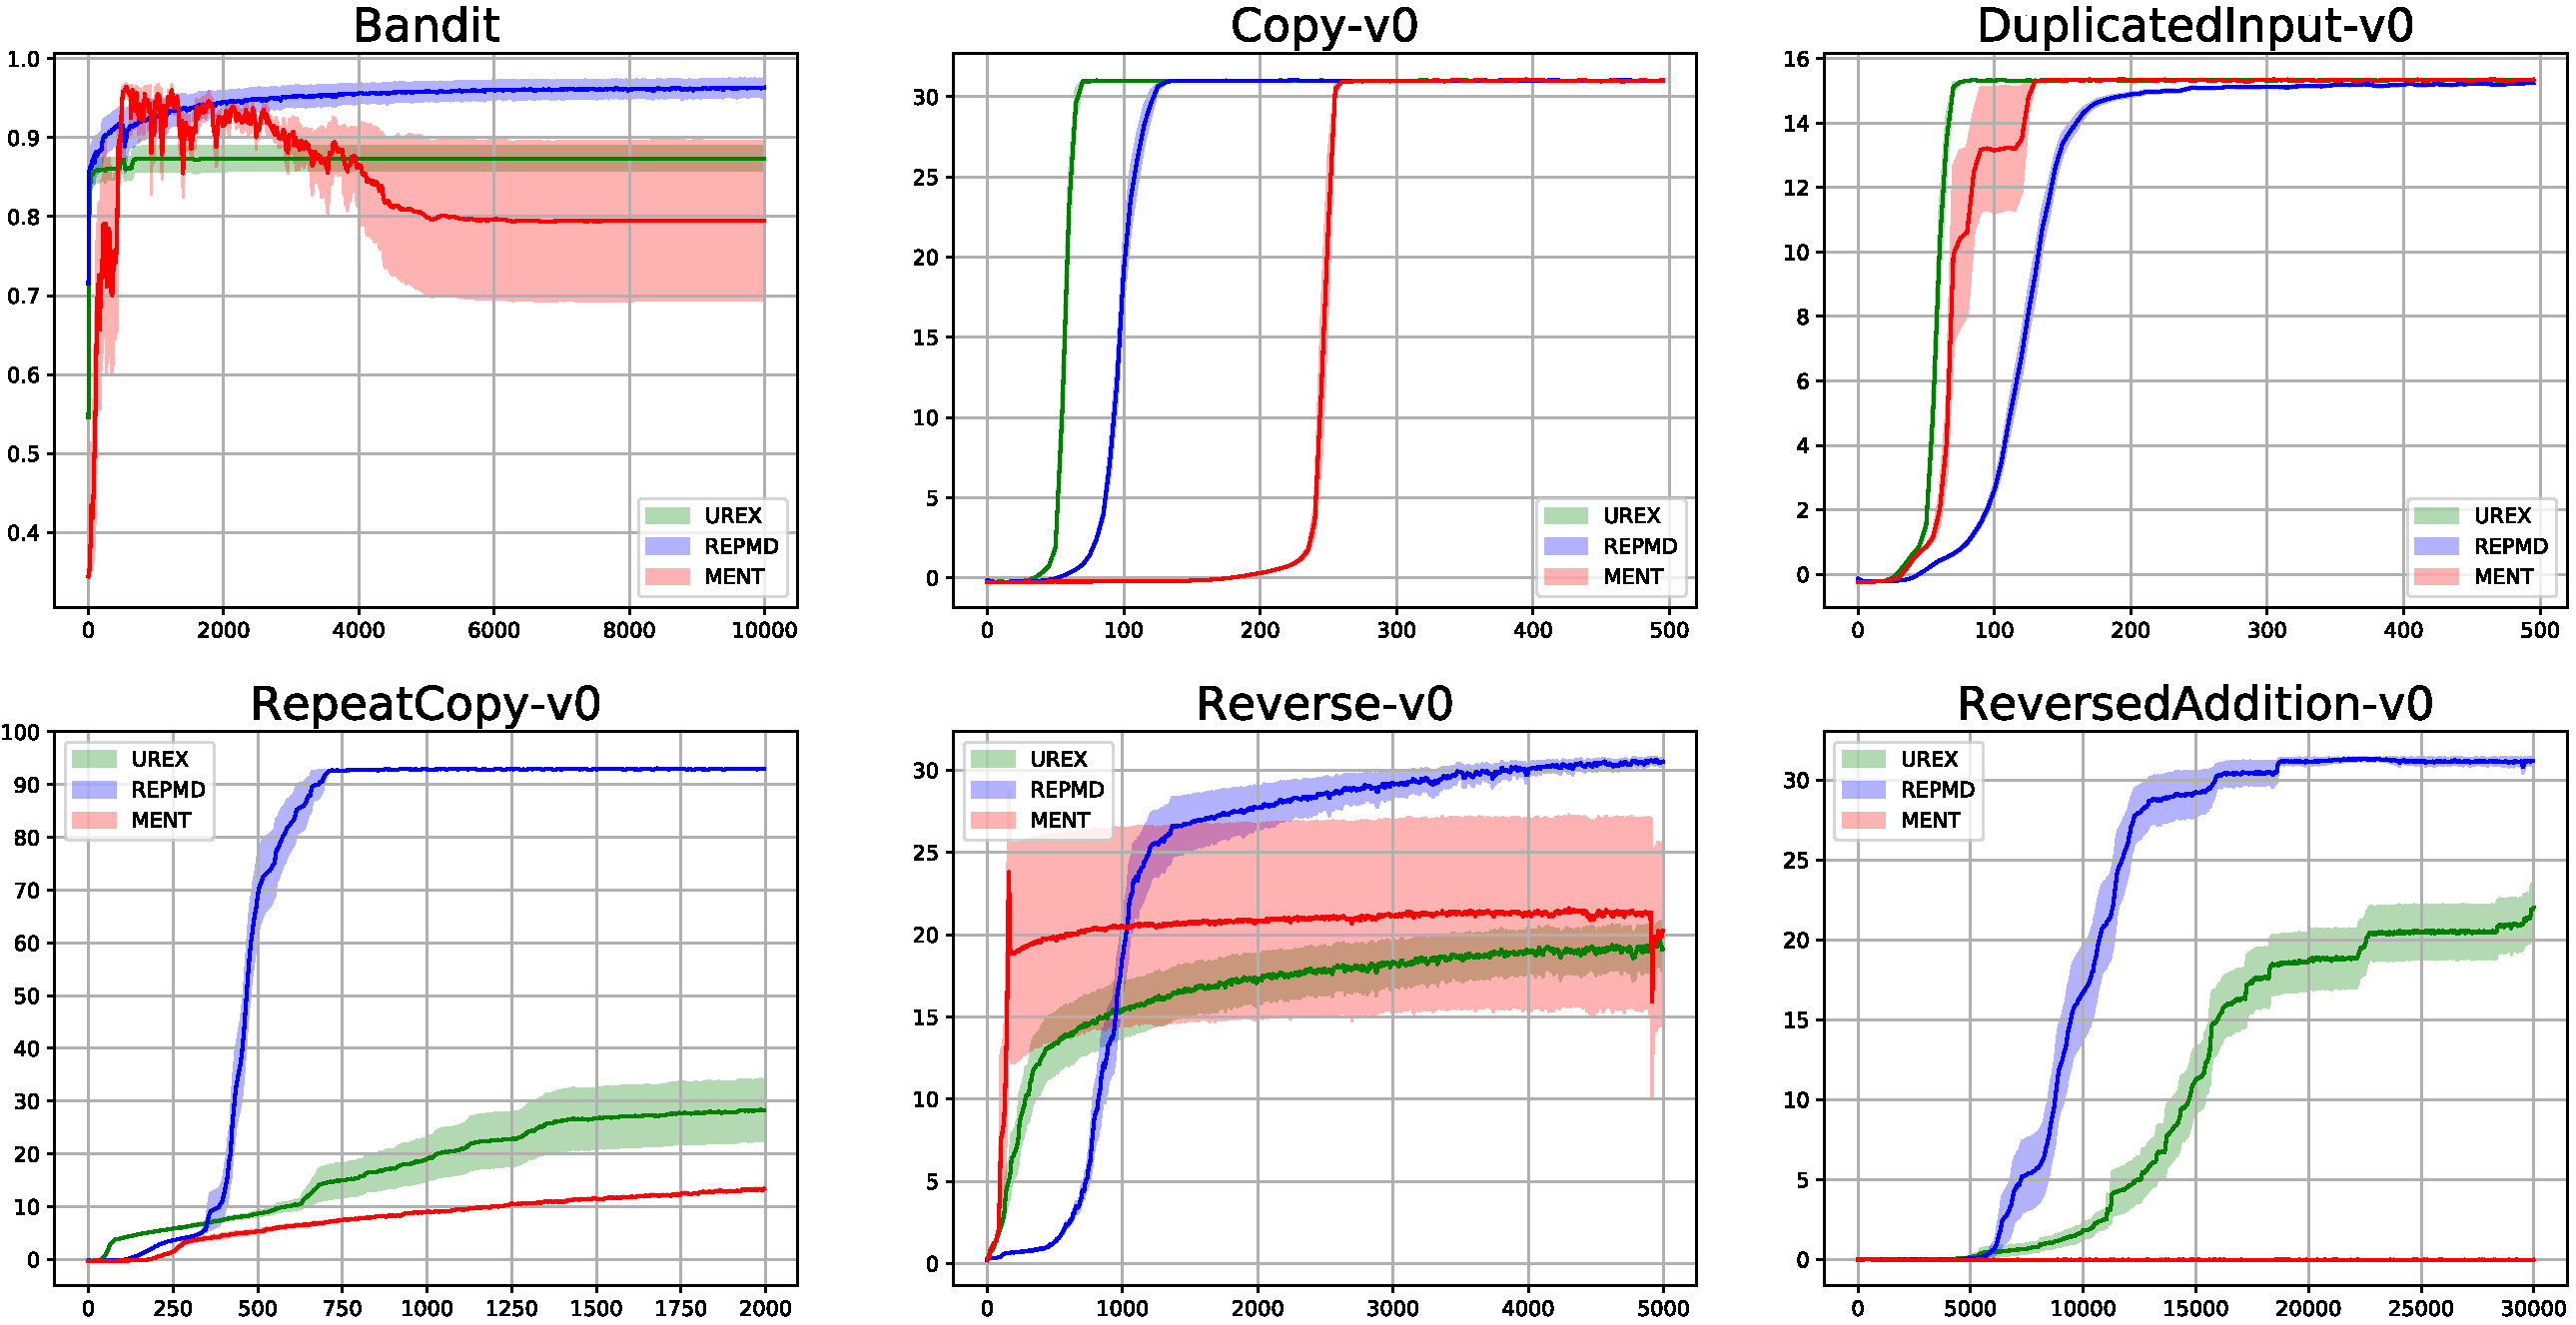
\includegraphics[width=0.85\linewidth]{./fig1.pdf}
\end{center}
\caption{
Results using the best hyper-parameters for each method: MENT (red), UREX (green), and REPMD (blue).
Plots show average reward with standard error during training. Synthetic bandit results averaged over 5 runs. Algorithmic task results averaged over 25 random training runs (5 runs $\times$ 5 random seeds for neural network initialization). X-axis is number of sampled trajectories. } 
\label{fig:results}
\end{figure*}

\subsection{Implementation Details}

As shown in \cref{alg:repmd}, the policy is updated by performing KL divergence projection using stochastic gradient descent (SGD). In our experiments, the end condition of SGD is controlled by two parameters: $\epsilon > 0$ and $\text{F\_STEP}\in \{0,1 \}$. First, SGD halts if the change of the KL divergence is below or equal to $\epsilon$. Second, $\text{F\_STEP}$ decides the maximum number of SGD steps. If $\text{F\_STEP}=1$, the maximum number is $\sqrt{t}$ at iteration $t$; while if $\text{F\_STEP}=0$, there is no restriction on the maximum number of gradient steps, and stopping condition of SGD only depends on $\epsilon$.

For the synthetic bandit problem, we explore the following main hyper-parameters: learning rate $\eta \in \{0.1, 0.01, 0.001\}$; entropy regularizer of UREX and MENT $\tau\in \{1.0, 0.5, 0.1, 0.05\}$; relative entropy regularizer of REPMD $\tau\in \{1.0, 0.5, 0.1, 0.05\}$; $\epsilon\in \{0.01, 0.005, 0.001\}$ and $\text{F\_STEP}\in \{0,1\}$ for the stop condition of SGD in REPMD. The entropy regularizer $\tau'$ of REPMD is set to 0.  

For the algorithmic tasks, $N$ distinct environments are used to generate samples. On each environment, $K$ random trajectories are sampled using the agent's policy to estimate gradient according to (\ref{eq:gradient_estimator}), which gives the batch size $N\times K$ in total. We apply the same batch training setting as in UREX \citep{nachum2017improving}, where $N=40$ and $K=10$. The following main hyper-parameters are explored: learning rate $\eta \in \{0.1, 0.01, 0.001\}$; relative entropy regularizer of REPMD $\tau\in \{1.0, 0.5, 0.1, 0.05\}$; entropy regularizer of REPMD $\tau'\in \{0, 0.01, 0.005, 0.001\}$; gradient clipped norm for training LSTM $c\in \{1, 10, 40, 100\}$; $\epsilon\in \{0.01, 0.005, 0.001\}$ and $\text{F\_STEP}\in \{0,1\}$ for the stopping condition of SGD in REPMD. Parameters of UREX are set according to the ones reported in \citet{nachum2017improving}. Implementations of all algorithm are based on the open source code by the author of UREX \footnote{\url{https://github.com/tensorflow/models/tree/master/research/pcl_rl}}.

\subsection{Comparative Evaluation}

For the synthetic bandit problem, we compare REPMD against REINFORCE with entropy regularization (MENT) \citep{williams1992simple} and under-appreciated reward exploration (UREX) \citep{nachum2017improving}. For the algorithmic tasks, we compare REPMD only against UREX, since UREX has been shown to outperform MENT in these cases \citep{nachum2017improving}. The results are reported in Figure (\ref{fig:results}). It is clear that REPMD substantially outperforms the competitors on all of these benchmark tasks. REPMD is able to consistently achieve the highest score and learn substantially faster than UREX. We also find the performance of UREX is very unstable. On the difficult tasks, including RepeatCopy, Reverse and ReversedAddition, UREX can only successfully find appropriate solutions a few times out of 5 runs for each random seed, which brings the overall scores down. This observation creates the gap between our presented results with the ones reported in the paper\footnote{The results reported in \citet{nachum2017improving} averages over 5 runs of random restart, while our results are averaged over 25 random training runs (5 runs $\times$ 5 random seed for neural network initialization). }. Note that the performance of REPMD is sill significantly better than UREX even compared with the results reported in \citet{nachum2017improving}. 

%\begin{wrapfigure}{R}{0.5\textwidth}
%\label{fig:ablation}
%  \begin{center}
%    \includegraphics[width=0.5\textwidth]{Copy.png}
%  \end{center}
%  \caption{Hello, Bye!}
%\end{wrapfigure}

\subsection{Ablation Study}

\piccaption[]{Ablation Study.\label{fig:ablation}}
\parpic[r]{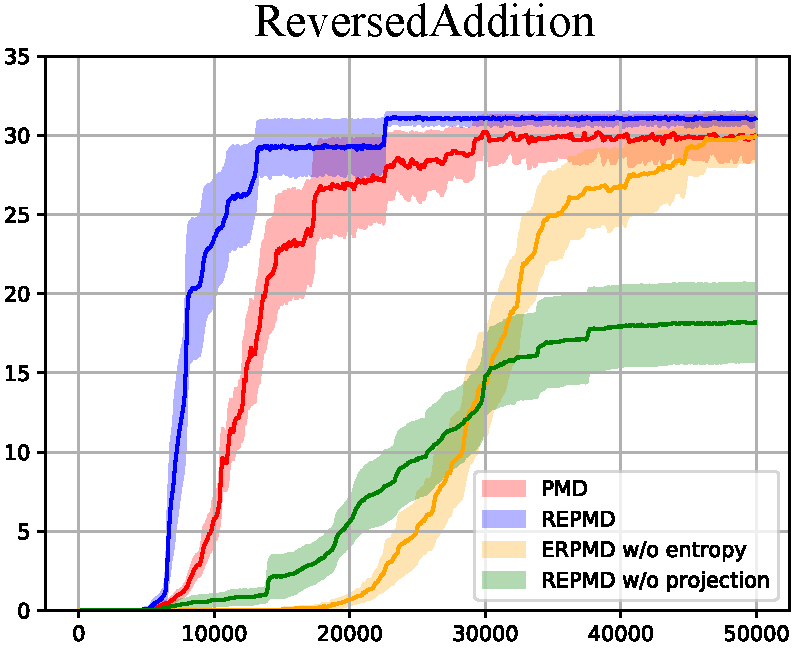
\includegraphics[width=0.35\linewidth]{ablation.pdf}}

\textbf{Importance of entropy regularizer.} The main difference between our objective \cref{eq:pmd} with the original MD is to add another entropy regularizer. We demonstrate the importance of this choice by presenting the results of REPMD with $\tau'=0$.

\textbf{Importance of KL divergence projection.} The main difference between REPMD and the UREX and MENT training methods is to use a projection step to optimize policy rather than performing a single gradient step. To show the importance of the projection step, we reimplement REPMD without projection, which only performs one step of gradient update at each iteration of training. 

\textbf{Importance of direction of KL divergence.} We implemented Policy Mirror Descent (PMD) as another baseline to prove the effectiveness of using the \emph{mean seeking} direction of KL divergence for policy optimization. Like in REPMD, we add a separate tempreture parameter $\tau'\geq 0$ to the original objective function (\ref{eq:max_expected_reward_plus_relative_entropy}) of PMD to encourage further exploration of the policy, which gives $\argmax_{\pi_\theta \in \Pi}{ \ep_{\rho \sim \pi_\theta}{  r(\rho)  - \tau \text{KL}(\pi_\theta \| \refPi) } + \tau'\cH(\pi_\theta) }$.

Results on ReversedAddition are reported in Figure (\ref{fig:ablation}). It clearly shows that optimizing policy by performing the \emph{mean seeking} KL divergence projection is very important as suggested in REPMD. 


\section{Conclusion and Future Work}
\label{sec:conclusion_and_future_work}

In this paper, we have proposed the reversed entropy policy mirror descent (REPMD) method for policy based reinforcement learning, which guarantees monotonic improvement in a well motivated objective. We show that the resulting method achieves better exploration than both a directed exploration method (UREX) and undirected maximum entropy exploration (MENT). It would be interesting to further extend the REPMD method within the actor-critic framework, by developing proper value function learning approach. %In particular, an actor-critic framework would also allow REPMD to perform important sampling on each step without heavy rollouts.



\section{Related Work}
\label{sec:related_work}

The lift-and-project approach is distinct from the previous literature on policy
search, with the exception of a few recent works:
Mirror Descent Guided Policy Search (MDGPS) \citep{montgomery2016guided},
Guide Actor-Critic (GAC) \citep{tangkaratt2017guide},
Maxmimum aposteriori (MPO) \citep{abdolmaleki2018maximum},
and Soft Actor-Critic (SAC) \citep{haarnoja2018soft}.
These approaches also adopt a mirror descent framework,
but differ from the proposed method in key aspects.
%
MDGPS \citep{montgomery2016guided} follows a different learning principle,
using the Lift Step to learn multiple local policies 
(rather than a single policy)
then aligning these with a global policy in the Project Step.
MDGPS also does not include the entropy term in the Lift objective,
which we have found to be essential for exploration. 
%
MPO \citep{abdolmaleki2018maximum} also neglects to add the additional entropy 
term;
\cref{subsec:ablationstudy} shows that entropy regularization with an
appropriate annealing of $\tau'$ significantly improves learning efficiency.
%
Both GAC and SAC use the mode seeking direction of KL divergence in
the Project Step, reversed from the mean seeking direction
we consider here \citep{tangkaratt2017guide,haarnoja2018soft}. 
Additionally, SAC only uses entropy regularization
in the Lift Step, neglecting the proximal relative entropy.
The benefits of regularizing with relative entropy
has been discussed in TRPO \citep{schulman2015trust}
and MPO \citep{abdolmaleki2018maximum},
where it is noted that proximal regularization
significantly improves learning stability.
GAC seeks to match the mean of Gaussian policies under second order approximation in the Project Step,
instead of directly minimizing the KL divergence with gradient descent.
%
Although one might also attempt to interpret ``one-step'' methods
in terms of lift-and-project,
these approaches would obliviously still differ from REPMD,
given that we use different directions of the KL divergence
for the Lift and Project steps respectively. 

Regarding the optimization objective,
several existing methods have considered related approaches,
either by considering (relative) entropy regularization during policy search,
or directly using KL divergence as the target objective. 
As noted in \cref{subsec:revisitTRPO},
REPMD resembles policy gradient methods that maximize expected reward
with an additional entropy regularizer
\citep{williams1991function,fox2015taming,nachum2017bridging}.
Using KL divergence, or Bregman divergences more generally,
as regularizers has also been explored
in \citet{liu2015finite,thomas2013projected,mahadevan2012sparse}.
However, these approaches differ from the proposed method
in important ways.
In particular, they apply regularization to the parameters of the
\emph{linear} approximated value functions, whereas here KL regularization
is applied directly to the policy space.
The literature on relative entropy policy search also uses a similar
KL divergence regularization scheme
\citep{peters2010relative,van2015learning},
but on joint state-action distributions.
Instead of KL divergence, Reward-Weighted Regression (RWR) uses
a log of the correlation between $\pi^*_\tau$ and $\pi_\theta$,
which is then approximated similar to a cross entropy loss
\citep{peters2007reinforcement,wierstra2008episodic}.

TRPO/PPO also has a similar formulation to
\cref{eq:max_expected_reward_plus_relative_entropy}
as a constrained version with a mean seeking KL divergence
\citep{schulman2015trust}. 
Unfortunately, the monotonic improvement guarantee only exists for an
impractical formulation of TRPO.%
%
\footnote{
For the monotonic improvement guarantee, % to hold,
TRPO must use $\KL^{\max} $ rather than the stanard KL divergence.
} 
Here, by contrast,
we use the lift-and-project reformulation to establish a monotonic
improvement guarantee in a simple and direct way.
Our proposed method also includes additional modifications that,
=======
\cite{schulman2015trust,schulman2017proximal}. 
Our proposed method includes additional modifications that,
>>>>>>> e0c8fb2d8e7529f9cc3150fdde9a95a20d888d9d
as shown in \cref{sec:experiments}, significantly improve performance.
UREX also uses the same mean seeking KL divergence for regularization,
which encourages exploration but also complicates the optimization;
as shown in \cref{sec:experiments},
UREX is significantly less efficient than the method proposed here.

Trust PCL adopts the same objective defined in \cref{eq:repmd},
including both entropy and relative entropy regularization
\citep{nachum2017trust}.
However, the policy update strategy is substantially different:
while REPMD uses KL projection, Trust PCL
minimizes a path inconsistency error (inherited from PCL)
between the value and policy along observed trajectories
\citep{nachum2017bridging}.
Although policy optimization by minimizing path inconsistency error
can efficiently utilize off-policy data, this approach loses the 
desirable monotonic improvement guarantee.

In terms of existing theoretical analyses, 
similar monotonic improvement guarantee exists for TRPO, but only for an
impractical formulation.%
%
\footnote{
	For the monotonic improvement guarantee to hold,
	TRPO must use $\KL^{\max} $ rather than the stanard KL divergence.
} 
Here, by contrast,
we use the lift-and-project reformulation to establish a monotonic
improvement guarantee in a simple and direct way.
MPO provides a guarantee on the regularized reward of a non-parametric policy,
but this depends on the assumption that a non-convex optimization problem
can be solved globally.
SAC obtains a similar result with respect to the optimal achievable
Q-values, again relying on an assumption that a non-convex optimization
problem can be solved globally.
We have shown that similar results hold in the case of PMD/REPMD,
but here we have also established something stronger:
When the projection step cannot be efficiently solved to global optimality,
we have shown that PMD/REPMD still preserve stationary points in 
their respective, principled objectives.
MPO and SAC have no such guarantee, as far as we are aware. 




\section{Conclusion and Future Work}
\label{sec:conclusion_and_future_work}

We have proposed reversed entropy policy mirror descent (REPMD)
as an effective new approach for policy based reinforcement learning
that also guarantees monotonic improvement in a well motivated objective.
We show that the resulting method achieves better exploration than both
a directed exploration strategy (UREX) and undirected maximum entropy
exploration (MENT). 
It will be interesting to further extend the follow-on
PMAC actor-critic framework
with further development of the value function learning approach.


\section*{Acknowledgements}
Part of the work has been done when the first two authors were interns in Borealis AI Lab. We gratefully acknowledge funding from Canada's Natural Sciences and Engineering Research Council (NSERC).

\bibliographystyle{named}
\bibliography{ijcai19}

\onecolumn
\appendix
\section{Proof of \cref{prop:mirrordescent_projection}}
\begin{proof}
	Note that $-\tau \KL(\pi_\theta \| \bar{\pi}_\tau^*) = - \tau \sum_{\rho}{ \pi_\theta(\rho) \log \pi_\theta(\rho) } + \tau \sum_{\rho}{ \pi_\theta(\rho) (\log \refPi(\rho) + r(\rho) / \tau ) }  - Z_{\refPi} = \ep_{\rho \sim \pi_\theta}{  r(\rho)  - \tau \KL(\pi_\theta \| \refPi) } - Z_{\refPi}$. Note the fact that $Z_{\refPi} \triangleq \tau \log{ \sum_{\rho}{\refPi(\rho) \exp\left\{ r(\rho) / \tau \right\} } }$ is indenpendent of $\pi_\theta$ given the reference policy $\refPi$.
\end{proof}
\section{Proof of \cref{prop:monoto_policymirrordescent}}
\label{appsec:monoto_policymirrordescent}
\begin{proof}
	{\bf (Monotonic Improvement Guarantee)} By the definition of $\pi_{\theta_{t+1}}$, note that $\KL(\pi_{\theta_{t+1}} \| \bar{\pi}_\tau^*)  = \min_{\pi_\theta \in \Pi}{ \KL(\pi_\theta \| \bar{\pi}_\tau^*)} \leq \KL(\pi_{\theta_{t}} \| \bar{\pi}_\tau^*)$. By expanding the KL divergence and rearranging terms, we have $ \tau \KL(\pi_{\theta_{t+1}} \| \pi_{\theta_{t}}) - \sum_{\rho}{ \pi_{\theta_{t+1}}(\rho) r(\rho) } \leq - \sum_{\rho}{ \pi_{\theta_{t}}(\rho) r(\rho) }$, which gives $\ep_{\rho \sim \pi_{\theta_{t+1}}}{  r(\rho)} - \ep_{\rho \sim \pi_{\theta_{t}}}{  r(\rho)} \geq \tau \KL(\pi_{\theta_{t+1}} \| \pi_{\theta_{t}}) \geq 0$.
	
	{\bf (Global optimum inclusion)}
\end{proof}
\section{Proof of \cref{thm:monotonically_increasing_sr_property}}
\begin{proof}
	Using $\KL(\bar{\pi}_{\tau,\tau^{\prime}}^* \| \pi_{\theta_{t+1}}) = \min_{\pi_\theta \in \Pi}{ \KL(\bar{\pi}_{\tau,\tau^{\prime}}^* \| \pi_\theta)} \le \KL(\bar{\pi}_{\tau,\tau^{\prime}}^* \| \pithetat)$ and Jensen's inequality,
	\begin{equation*}
	\begin{split}
	&\SR(\pi_{\theta_{t+1}}) - \SR(\pithetat) = (\tau + \tau^{\prime}) \log{ \sum\limits_{\rho}{ \frac{  \exp\left\{ \frac{r(\rho) + \tau \log{\pi_{\theta_{t+1}}(\rho)} }{\tau + \tau^{\prime}} \right\}  }{ \sum\limits_{\rho}{  \exp\left\{ \frac{r(\rho) + \tau \log{\pithetat(\rho)} }{\tau + \tau^{\prime}} \right\} } }  } } \\
	=& (\tau + \tau^{\prime}) \log{ \sum\limits_{\rho}{ \frac{  \exp\left\{ \frac{r(\rho) + \tau \log{\pithetat(\rho)} }{\tau + \tau^{\prime}} \right\}  }{ \sum\limits_{\rho}{  \exp\left\{ \frac{r(\rho) + \tau \log{\pithetat(\rho)} }{\tau + \tau^{\prime}} \right\} } }  } \cdot \exp\left\{ \frac{\tau \log{\pi_{\theta_{t+1}}(\rho)} - \tau \log{\pithetat(\rho)} }{\tau + \tau^{\prime}} \right\} } \\
	=& (\tau + \tau^{\prime}) \log{ \sum\limits_{\rho}{ \bar{\pi}_{\tau,\tau^{\prime}}^*(\rho) } \cdot \exp\left\{ \frac{\tau \log{\pi_{\theta_{t+1}}(\rho)} - \tau \log{\pithetat(\rho)} }{\tau + \tau^{\prime}} \right\} } \\
	\ge& (\tau + \tau^{\prime}) \sum\limits_{\rho}{ \bar{\pi}_{\tau,\tau^{\prime}}^*(\rho) \log{ \exp\left\{ \frac{\tau \log{\pi_{\theta_{t+1}}(\rho)} - \tau \log{\pithetat(\rho)} }{\tau + \tau^{\prime}} \right\} } } \\
	=& \tau \sum\limits_{\rho}{ \bar{\pi}_{\tau,\tau^{\prime}}^*(\rho) \log{ \frac{\pi_{\theta_{t+1}}(\rho)}{\pithetat(\rho)} } } = \tau \left[ \KL(\bar{\pi}_{\tau,\tau^{\prime}}^* \| \pithetat) - \KL(\bar{\pi}_{\tau,\tau^{\prime}}^* \| \pi_{\theta_{t+1}})\right] \ge 0. \qedhere
	\end{split}
	\end{equation*}
\end{proof}

\section{Proof of \cref{prop:solvableprojection}}
\section{Proof of \cref{prop:sr}}
\begin{proof}
	To prove (i), note that as $\tau \to 0$, $\SR(\pi_\theta) \to \tau^{\prime} \log{ \sum_{\rho}{ \exp\left\{ \frac{r(\rho) }{ \tau^{\prime} } \right\} }}$, the standard softmax value. Taking limit on $\tau'$ gives the hardmax value $\max_{\rho}{r(\rho)}$ as $\tau^{\prime} \to 0$.
	
	To prove (ii), we have 
	\begin{align*}
	&\lim\limits_{\tau \to \infty}{ (\tau + \tau^{\prime})\log{ \sum_{\rho}{ \exp\left\{ \frac{r(\rho) + \tau \log{\pi_\theta(\rho)} }{\tau + \tau^{\prime}} \right\} }} } = {\scalebox{.95} {$\lim\limits_{\tau \to \infty}{ \frac{ \sum_{\rho}{ \pi_\theta(\rho) \exp\{ \frac{r(\rho) - \tau^{\prime} \log{\pi_\theta(\rho)} }{\tau + \tau^{\prime}} \} \left( r(\rho) - \tau^{\prime}\log{\pi_\theta(\rho)} \right) } }{  \sum_{\rho}{ \pi_\theta(\rho) \exp\{ \frac{r(\rho) - \tau^{\prime} \log{\pi_\theta(\rho)} }{\tau + \tau^{\prime}} \} } } }$ } }\\
	&= \sum_{\rho}{ \pi_\theta(\rho) \left[ r(\rho) - \tau^{\prime}\log{\pi_\theta(\rho)} \right] } = \ep_{\rho \sim \pi_\theta}{r(\rho)} + \tau^{\prime} \mathcal{H}(\pi_\theta)
	\end{align*}
	As $\tau^{\prime} \to 0$, $\SR(\pi_\theta) \to \ep_{\rho \sim \pi_\theta}{r(\rho)}$.
\end{proof}

\section{Proof for Section ***}
\begin{lem}
	\label{lem:opt_pi_ref}
	The lift step of \cref{eq:repmd} has the following closed form expression:
	\begin{equation*}
	\bar{\pi}_{\tau,\tau^{\prime}}^*(\rho) \triangleq \frac{\refPi(\rho) \exp\left\{ \frac{r(\rho)-\tau^{\prime} \log \refPi(\rho) }{ \tau+\tau^{\prime}} \right\}}{ \sum_{\rho^{\prime}}{\refPi(\rho^{\prime}) \exp\left\{ \frac{r(\rho^{\prime})-\tau^{\prime} \log \refPi(\rho^{\prime})}{ \tau+\tau^{\prime}} \right\} } }.
	\end{equation*}
\end{lem}
\begin{proof}
	Rewrite the objective function defined in \cref{eq:repmd},
	\begin{equation}
	\ep\limits_{\rho \sim \pi} r(\rho)  - \tau \KL(\pi \| \refPi) + \tau^{\prime} \cH(\pi) = \ep\limits_{\rho \sim \pi} [r(\rho) + \tau \log \refPi(\rho)] + (\tau+\tau^{\prime}) \cH(\pi),
	\end{equation}
	which is an entropy regularized reshaped reward objective. The optimal policy of this objective can be obtained by directly applying Lemma 4 of \citet{nachum2017bridging}, i.e.
	\begin{equation}
	\label{pi_bar_star_tau_tauprime_prop_form}
	\bar{\pi}_{\tau,\tau^{\prime}}^*(\rho)\propto \exp\left\{ \frac{r(\rho)+\tau \log \refPi(\rho)}{\tau+\tau^{\prime}} \right\} = \refPi(\rho) \exp\left\{ \frac{r(\rho)-\tau^{\prime} \log \refPi(\rho)}{\tau+\tau^{\prime}} \right\}. \qedhere
	\end{equation}
\end{proof}

\section{Proof of \cref{thm:repmdgradientestimate}}
\begin{proof}
	Note that
	\begin{equation*}
	\label{eq:importance_sampling_kl}
	\KL(\bar{\pi}_{\tau,\tau^{\prime}}^* \| \pi_\theta) = \ep_{\rho \sim \bar{\pi}_{\tau,\tau^{\prime}}^* } \left[ \log \bar{\pi}_{\tau,\tau^{\prime}}^*(\rho) - \log \pi_\theta(\rho) \right] = \ep_{\rho\sim \refPi} \left[  \frac{\bar{\pi}_{\tau,\tau^{\prime}}^*(\rho)}{\refPi(\rho)} \left(\log \bar{\pi}_{\tau,\tau^{\prime}}^*(\rho) - \log \pi_\theta(\rho) \right) \right].
	\end{equation*}	
	%	We can draw $K$ \textit{i.i.d.} samples $\{\rho_1, \dots, \rho_K\}$ from the \emph{reference policy} $\refPi$, and then approximate the gradient of $\KL(\bar{\pi}_{\tau,\tau^{\prime}}^* \| \pi_\theta)$ by averaging these $K$ samples according to \cref{eq:importance_sampling_kl}. 
	Therefore, taking gradient on both sides,
	\begin{equation}
	\begin{split}
	&\nabla_{\theta} \KL(\bar{\pi}_{\tau,\tau^{\prime}}^* \| \pi_\theta) \approx -\frac{1}{K}\sum_{k=1}^K \frac{\bar{\pi}_{\tau,\tau^{\prime}}^* (\rho_k)}{\refPi(\rho_k)} \nabla_{\theta} \log \pi_\theta(\rho_k) \\ 
	\approx & -\frac{1}{K}\sum_{k=1}^K \frac{\exp \{\omega_k\}} {\frac{1}{K} \sum_{j=1}^K \exp \{\omega_j\}} \nabla_{\theta} \log \pi_\theta(\rho_k) =  -\sum\limits_{k=1}^K{ \frac{ \exp\left\{ \omega_k \right\} }{ \sum_{j=1}^K{ \exp\left\{ \omega_j \right\}}} \nabla_{\theta} \log{\pi_\theta(\rho_k)} } \qedhere.
	\end{split}
	\end{equation}
	\todor[]{More details}
\end{proof}

\section{Stochastic Transition Setting}

In \cref{sec:notations_and_settings}, we assume that the state transition function is deterministic for simplicity. For completeness, we consider the general stochastic transition setting here.

\subsection{Notations and Settings}

Recall in \cref{sec:notations_and_settings}, the policy probability of trajectory $\rho=(s_1, a_1, \dots, a_{T-1}, s_T)$ is denoted as $\pi(\rho) = \prod_{t=1}^{T-1} \pi(a_t| s_t)$. We define transition probability of $\rho$ as $f(\rho) \triangleq \prod_{t=1}^{T-1}{ f(s_{s+1} | s_t, a_t)}$. The total probability of $\rho$ under policy $\pi$ and transition $f$ is then $p_{\pi, f}(\rho) \triangleq \pi(\rho) f(\rho) = \prod_{t=1}^{T-1}{ \pi(a_t | s_t) f(s_{s+1} | s_t, a_t)}$. We use $\Delta_{f} \triangleq \{ \pi | \sum_{\rho}{ p_{\pi, f}(\rho) } = \sum_{\rho}{\pi(\rho) f(\rho)} = 1, \pi(\rho) \ge 0, f(\rho) > 0, \forall \rho \}$ to refer to the probabilistic simplex over all possible trajectories. It is obvious that $p_{\pi, f}(\rho) = \pi(\rho)$ and $\Delta_f = \Delta$ under deterministic transition setting, i.e., $f(\rho) = 1, \forall \rho$.

\subsection{REPMD Optimization Problem}

The proposed REPMD algorithm solves \cref{eq:repmd} in the deterministic transition setting. In the stochastic setting, the corresponding problem is,
\begin{equation}
\label{eq:repmd_stochastic}
\begin{split}
	&\argmin\limits_{\pi_\theta \in \Pi}{\KL(p_{\bar{\pi}_{\tau,\tau^{\prime}}^*, f}  \| p_{\pi_\theta, f} ) }, \\
	\text{where}\ \ \bar{\pi}_{\tau,\tau^{\prime}}^* & =  \argmax\limits_{\pi \in \Delta_f}{ \ep\limits_{\rho \sim p_{\pi, f}}{ \left[ r(\rho) - \tau^{\prime} \log{\pi(\rho)} \right] } - \tau \KL(p_{\pi, f} \| p_{\pi_{\theta_t}, f} ) },
\end{split}
\end{equation}
which also recovers \cref{eq:repmd} as a special case when $f(\rho) = 1, \forall \rho$.

Like \cref{eq:repmd}, $\bar{\pi}_{\tau,\tau^{\prime}}^*$ in \cref{eq:repmd_stochastic} also has a closed form expression,
\begin{lem}
\label{lem:opt_pi_ref_stochastic}
The unconstrained optimal policy of \cref{eq:repmd_stochastic} has the following closed form expression:
\begin{equation*}
	\bar{\pi}_{\tau,\tau^{\prime}}^*(\rho) \triangleq \frac{\refPi(\rho) \exp\left\{ \frac{r(\rho)-\tau^{\prime} \log \refPi(\rho) }{ \tau+\tau^{\prime}} \right\}}{ \sum_{\rho^{\prime}}{\refPi(\rho^{\prime}) f(\rho^{\prime}) \exp\left\{ \frac{r(\rho^{\prime})-\tau^{\prime} \log \refPi(\rho^{\prime})}{ \tau+\tau^{\prime}} \right\} } }.
\end{equation*}
\end{lem}
\begin{proof}
Rewrite the maximization problem in \cref{eq:repmd_stochastic} as (take $\pi_{\theta_t}$ as the reference policy $\refPi$),
\begin{equation*}
\begin{split}
	\textmax\limits_{\pi}&{ \sum\limits_{\rho}{ \pi(\rho) f(\rho) \left[ r(\rho)  - \left( \tau + \tau^{\prime} \right) \log{\pi(\rho)} + \tau \log{\bar{\pi}(\rho)} \right]} } \\
	\st &\sum\limits_{\rho}{ \pi(\rho) f(\rho)} = 1.
\end{split}
\end{equation*}
The KKT condition of the above problem is,
\begin{equation*}
\begin{split}
	f(\rho) \left[ r(\rho) - \left( \tau + \tau^{\prime} \right) \log{\pi(\rho)} + \tau \log{\bar{\pi}(\rho)} +  \lambda - \left( \tau + \tau^{\prime} \right) \right] &= 0, \ \forall \rho \\
	\sum\limits_{\rho}{ \pi(\rho) f(\rho)} &= 1.
\end{split}
\end{equation*}
Using $f(\rho) > 0, \forall \rho$ and solving the KKT condition, we obtain the expression of $\bar{\pi}_{\tau,\tau^{\prime}}^*$.
\end{proof}

Lemma \ref{lem:opt_pi_ref_stochastic} recovers Lemma \ref{lem:opt_pi_ref} as a special case when $f(\rho) = 1, \forall \rho$.

\subsection{Theoretical Analysis}

In stochastic transition setting, we define the follow softmax approximated expected reward of $\pi_\theta$
\begin{equation*}
	\SR_f(\pi_\theta) \triangleq (\tau + \tau^{\prime})\log{ \sum_{\rho}{ f(\rho) \exp\left\{ \frac{r(\rho) + \tau \log{\pi_\theta(\rho)} }{\tau + \tau^{\prime}} \right\} }},
\end{equation*}
which recovers $\SR(\pi_\theta)$ when $f(\rho) = 1, \forall \rho$. The monotonic improvement property is for $\SR_f(\pi_\theta)$.

\begin{thm}
\label{thm:monotonically_increasing_sr_property_stochastic}
Assume that $\pi_{\theta_{t}}$ is the update sequence of the REPMD algorithm in \cref{eq:repmd_stochastic}, then
\begin{equation*}
	\SR_f(\pi_{\theta_{t+1}}) - \SR_f(\pithetat)\ge 0.
\end{equation*}
\end{thm}
\begin{proof}
	Using $\KL(p_{\bar{\pi}_{\tau,\tau^{\prime}}^*, f} \| p_{\pi_{\theta_{t+1}}, f}) = \min_{\pi_\theta \in \Pi}{ \KL(p_{\bar{\pi}_{\tau,\tau^{\prime}}^*, f}  \| p_{\pi_\theta, f} ) } \le \KL(p_{\bar{\pi}_{\tau,\tau^{\prime}}^*, f} \| p_{\pithetat, f})$ and Jensen's inequality,
	\begin{equation*}
	\begin{split}
	&\SR_f(\pi_{\theta_{t+1}}) - \SR_f(\pithetat) = (\tau + \tau^{\prime}) \log{ \sum\limits_{\rho}{ \frac{ f(\rho) \exp\left\{ \frac{r(\rho) + \tau \log{\pi_{\theta_{t+1}}(\rho)} }{\tau + \tau^{\prime}} \right\}  }{ \sum\limits_{\rho}{ f(\rho) \exp\left\{ \frac{r(\rho) + \tau \log{\pithetat(\rho)} }{\tau + \tau^{\prime}} \right\} } }  } } \\
	=& (\tau + \tau^{\prime}) \log{ \sum\limits_{\rho}{ \frac{ f(\rho) \exp\left\{ \frac{r(\rho) + \tau \log{\pithetat(\rho)} }{\tau + \tau^{\prime}} \right\}  }{ \sum\limits_{\rho}{ f(\rho) \exp\left\{ \frac{r(\rho) + \tau \log{\pithetat(\rho)} }{\tau + \tau^{\prime}} \right\} } }  } \cdot \exp\left\{ \frac{\tau \log{\pi_{\theta_{t+1}}(\rho)} - \tau \log{\pithetat(\rho)} }{\tau + \tau^{\prime}} \right\} } \\
	=& (\tau + \tau^{\prime}) \log{ \sum\limits_{\rho}{ \bar{\pi}_{\tau,\tau^{\prime}}^*(\rho) f(\rho) } \cdot \exp\left\{ \frac{\tau \log{\pi_{\theta_{t+1}}(\rho)} - \tau \log{\pithetat(\rho)} }{\tau + \tau^{\prime}} \right\} } \\
	\ge& (\tau + \tau^{\prime}) \sum\limits_{\rho}{ \bar{\pi}_{\tau,\tau^{\prime}}^*(\rho) f(\rho) \cdot \log{ \exp\left\{ \frac{\tau \log{\pi_{\theta_{t+1}}(\rho)} - \tau \log{\pithetat(\rho)} }{\tau + \tau^{\prime}} \right\} } } \\
	=& \tau \sum\limits_{\rho}{ \bar{\pi}_{\tau,\tau^{\prime}}^*(\rho) f(\rho) \cdot \log{ \frac{\pi_{\theta_{t+1}}(\rho)}{\pithetat(\rho)} } } \\
	=& \tau \sum\limits_{\rho}{ \bar{\pi}_{\tau,\tau^{\prime}}^*(\rho) f(\rho) \cdot \log{ \frac{ \pi_{\theta_{t+1}}(\rho) f(\rho) }{ \pithetat(\rho) f(\rho)} } } \\
	=& \tau \left[ \KL(p_{\bar{\pi}_{\tau,\tau^{\prime}}^*, f} \| p_{\pithetat, f}) - \KL(p_{\bar{\pi}_{\tau,\tau^{\prime}}^*, f} \| p_{\pi_{\theta_{t+1}}, f}) \right] \ge 0. \qedhere
	\end{split}
	\end{equation*}
\end{proof}

$\SR_f(\pi_\theta)$ also recovers corresponding performance measures in the stochastic transition setting.
\begin{prop}
\label{prop:sr_stochastic}
$\SR_f(\pi_\theta)$ satisfies the following properties:
\begin{enumerate}[label=(\roman*)]
	\item  $\SR_f(\pi_\theta) \to \max_{\rho}{r(\rho)}$, as $\tau \to 0, \tau^{\prime} \to 0$.
	\item $\SR_f(\pi_\theta) \to \ep\limits_{\rho \sim p_{\pi_\theta, f}}{r(\rho)}$, as $\tau \to \infty, \tau^{\prime} \to 0$. 
\end{enumerate}	
\end{prop}
\begin{proof}
To prove (i), note that as $\tau \to 0$, $\SR_f(\pi_\theta) \to \tau^{\prime} \log{ \sum_{\rho}{ f(\rho) \exp\left\{ \frac{r(\rho) }{ \tau^{\prime} } \right\} }}$. Taking limit on $\tau'$ gives the hardmax value $\max_{\rho}{r(\rho)}$ as $\tau^{\prime} \to 0$.
	
To prove (ii), we have 
\begin{align*}
	&\lim\limits_{\tau \to \infty}{ (\tau + \tau^{\prime})\log{ \sum_{\rho}{ f(\rho) \exp\left\{ \frac{r(\rho) + \tau \log{\pi_\theta(\rho)} }{\tau + \tau^{\prime}} \right\} }} } \\
	=& \lim\limits_{\tau \to \infty}{ \frac{ \sum_{\rho}{ \pi_\theta(\rho) f(\rho) \exp\{ \frac{r(\rho) - \tau^{\prime} \log{\pi_\theta(\rho)} }{\tau + \tau^{\prime}} \} \left( r(\rho) - \tau^{\prime}\log{\pi_\theta(\rho)} \right) } }{  \sum_{\rho}{ \pi_\theta(\rho) f(\rho) \exp\{ \frac{r(\rho) - \tau^{\prime} \log{\pi_\theta(\rho)} }{\tau + \tau^{\prime}} \} } } } \\
	=& \sum_{\rho}{ \pi_\theta(\rho) f(\rho) \left[ r(\rho) - \tau^{\prime}\log{\pi_\theta(\rho)} \right] } = \ep\limits_{\rho \sim p_{\pi_\theta, f}}{r(\rho)} -  \tau^{\prime} \cdot \ep\limits_{\rho \sim p_{\pi_\theta, f}}{  \log{\pi_\theta(\rho)} }
\end{align*}
As $\tau^{\prime} \to 0$, $\SR_f(\pi_\theta) \to \ep_{\rho \sim p_{\pi_\theta, f}}{r(\rho)}$.
\end{proof}

\subsection{Learning}

The REPMD learning process is intact under the stochastic transition setting. Similar with \cref{eq:importance_sampling_kl}, we can estimate the KL divergence in the projection step of \cref{eq:repmd_stochastic} by drawing $K$ \textit{i.i.d.} samples $\{\rho_1, \dots, \rho_K\}$ from $p_{\refPi, f}$, i.e., the mixture of $\refPi$ and $f$, which is exactly the process of sampling from $\refPi$ and interacting with the environment,
\begin{equation}
\label{eq:importance_sampling_kl_stochastic}
\begin{split}
	\KL(p_{\bar{\pi}_{\tau,\tau^{\prime}}^*, f}  \| p_{\pi_\theta, f} ) &= \ep_{\rho \sim p_{\bar{\pi}_{\tau,\tau^{\prime}}^*, f} } \left[ \log \bar{\pi}_{\tau,\tau^{\prime}}^*(\rho) - \log \pi_\theta(\rho) \right] \\
	&= \ep_{\rho\sim p_{\refPi, f}} \frac{\bar{\pi}_{\tau,\tau^{\prime}}^*(\rho)}{\refPi(\rho)} \left[ \log \bar{\pi}_{\tau,\tau^{\prime}}^*(\rho) - \log \pi_\theta(\rho) \right].
\end{split}
\end{equation}

We can then approximate the gradient of $\KL(p_{\bar{\pi}_{\tau,\tau^{\prime}}^*, f}  \| p_{\pi_\theta, f} )$ by averaging these $K$ samples according to \cref{eq:importance_sampling_kl_stochastic}. 

\begin{thm}
\label{thm:repmdgradientestimate_stochastic}
Let $\omega_k = \frac{r(\rho_k) - \tau^{\prime} \log{\refPi(\rho_k)} }{\tau + \tau^{\prime}}$. Given $K$ \emph{i.i.d.} samples $\{\rho_1, \dots, \rho_K\}$ from the \emph{reference policy} $\refPi$, we have the following unbiased gradient estimator,
\begin{equation}
	\nabla_{\theta} \KL(p_{\bar{\pi}_{\tau,\tau^{\prime}}^*, f}  \| p_{\pi_\theta, f} ) \approx -\sum\limits_{k=1}^K{ \frac{ \exp\left\{ \omega_k \right\} }{ \sum_{j=1}^K{ \exp\left\{ \omega_j \right\}}} \nabla_{\theta} \log{\pi_\theta(\rho_k)} },
\end{equation}
\end{thm}
\begin{proof}
See Theorem \ref{thm:repmdgradientestimate}.
\end{proof}




\end{document}

